\section{Demonstration}

    \subsection{An colorful approach}

        Suppose we have the following transformation (Figure~\ref{simple01}).
        
        % \begin{figure}[ht]
        %     \caption{A simple transformation.}
        %     \label{simple01}
        %     \centering
        %     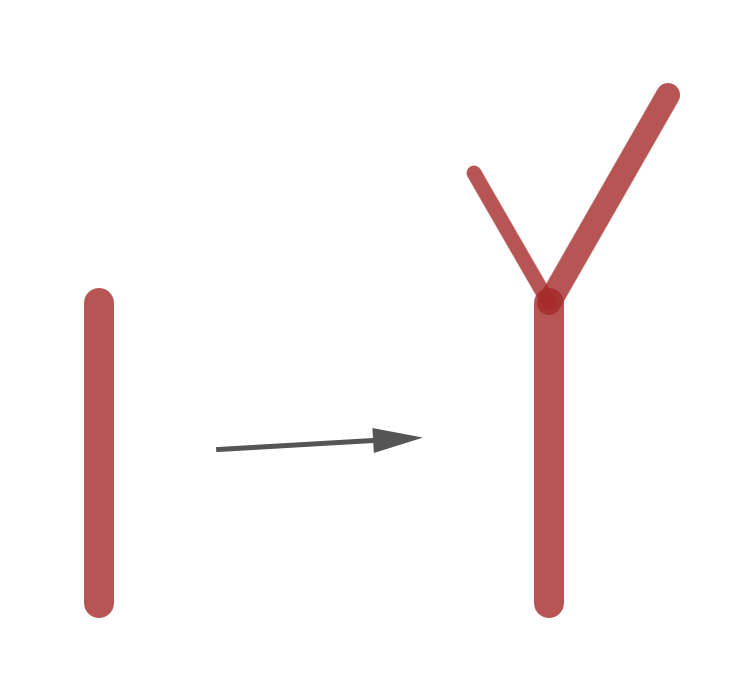
\includegraphics[width=0.15\textwidth]{img/simple01.png}
        % \end{figure}
        % \FloatBarrier

        That is, transform a segment into a branch composed of three segments.
        This process can be applied to the two smaller branches.
        Repeating this process some numbers of times reveals a beautiful, fractal pattern (Figure~\ref{simple02}).
        This pattern is very similar to the \emph{Barnsley fern} \cite{barnsley_fern}.

        \begin{figure}[ht]
            \centering
            \caption{First steps.}
            \subcaptionbox{\label{simple01} A simple transformation.}[0.45\textwidth]
                {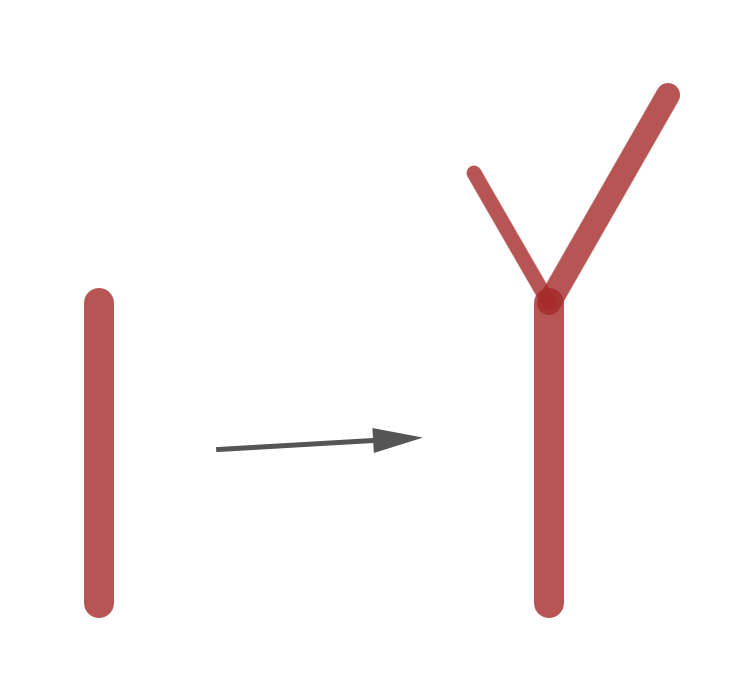
\includegraphics[width=0.2\textwidth]{img/simple01.png}}
            ~
            \subcaptionbox{\label{simple02} Several level of recursion.}[0.45\textwidth]
                {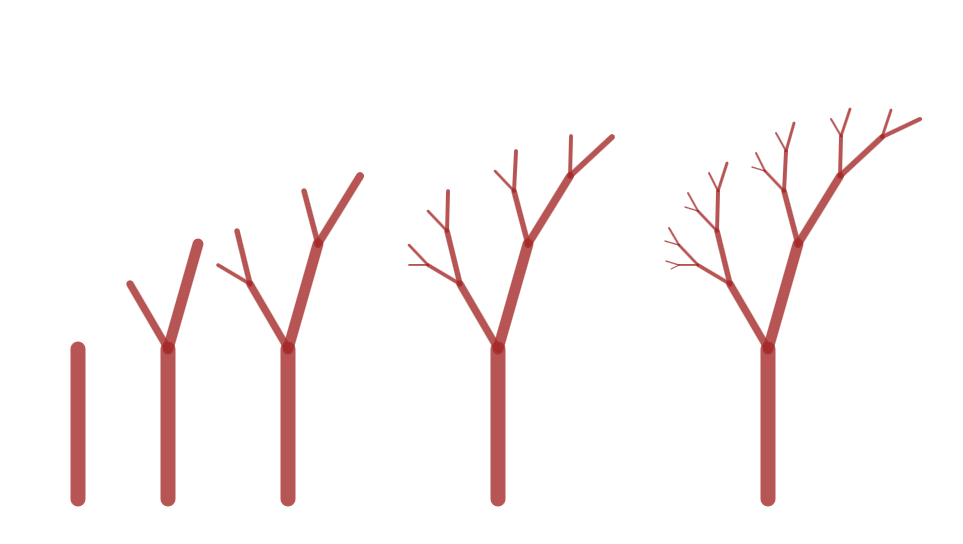
\includegraphics[width=0.4\textwidth]{img/simple02.png}}            
        \end{figure}
        \FloatBarrier

        A much more detailed rendering can be observed in Figure~\ref{simple03}

        \begin{figure}[ht]
            \caption{\label{simple03} A deeper recursion level.}
            \centering
            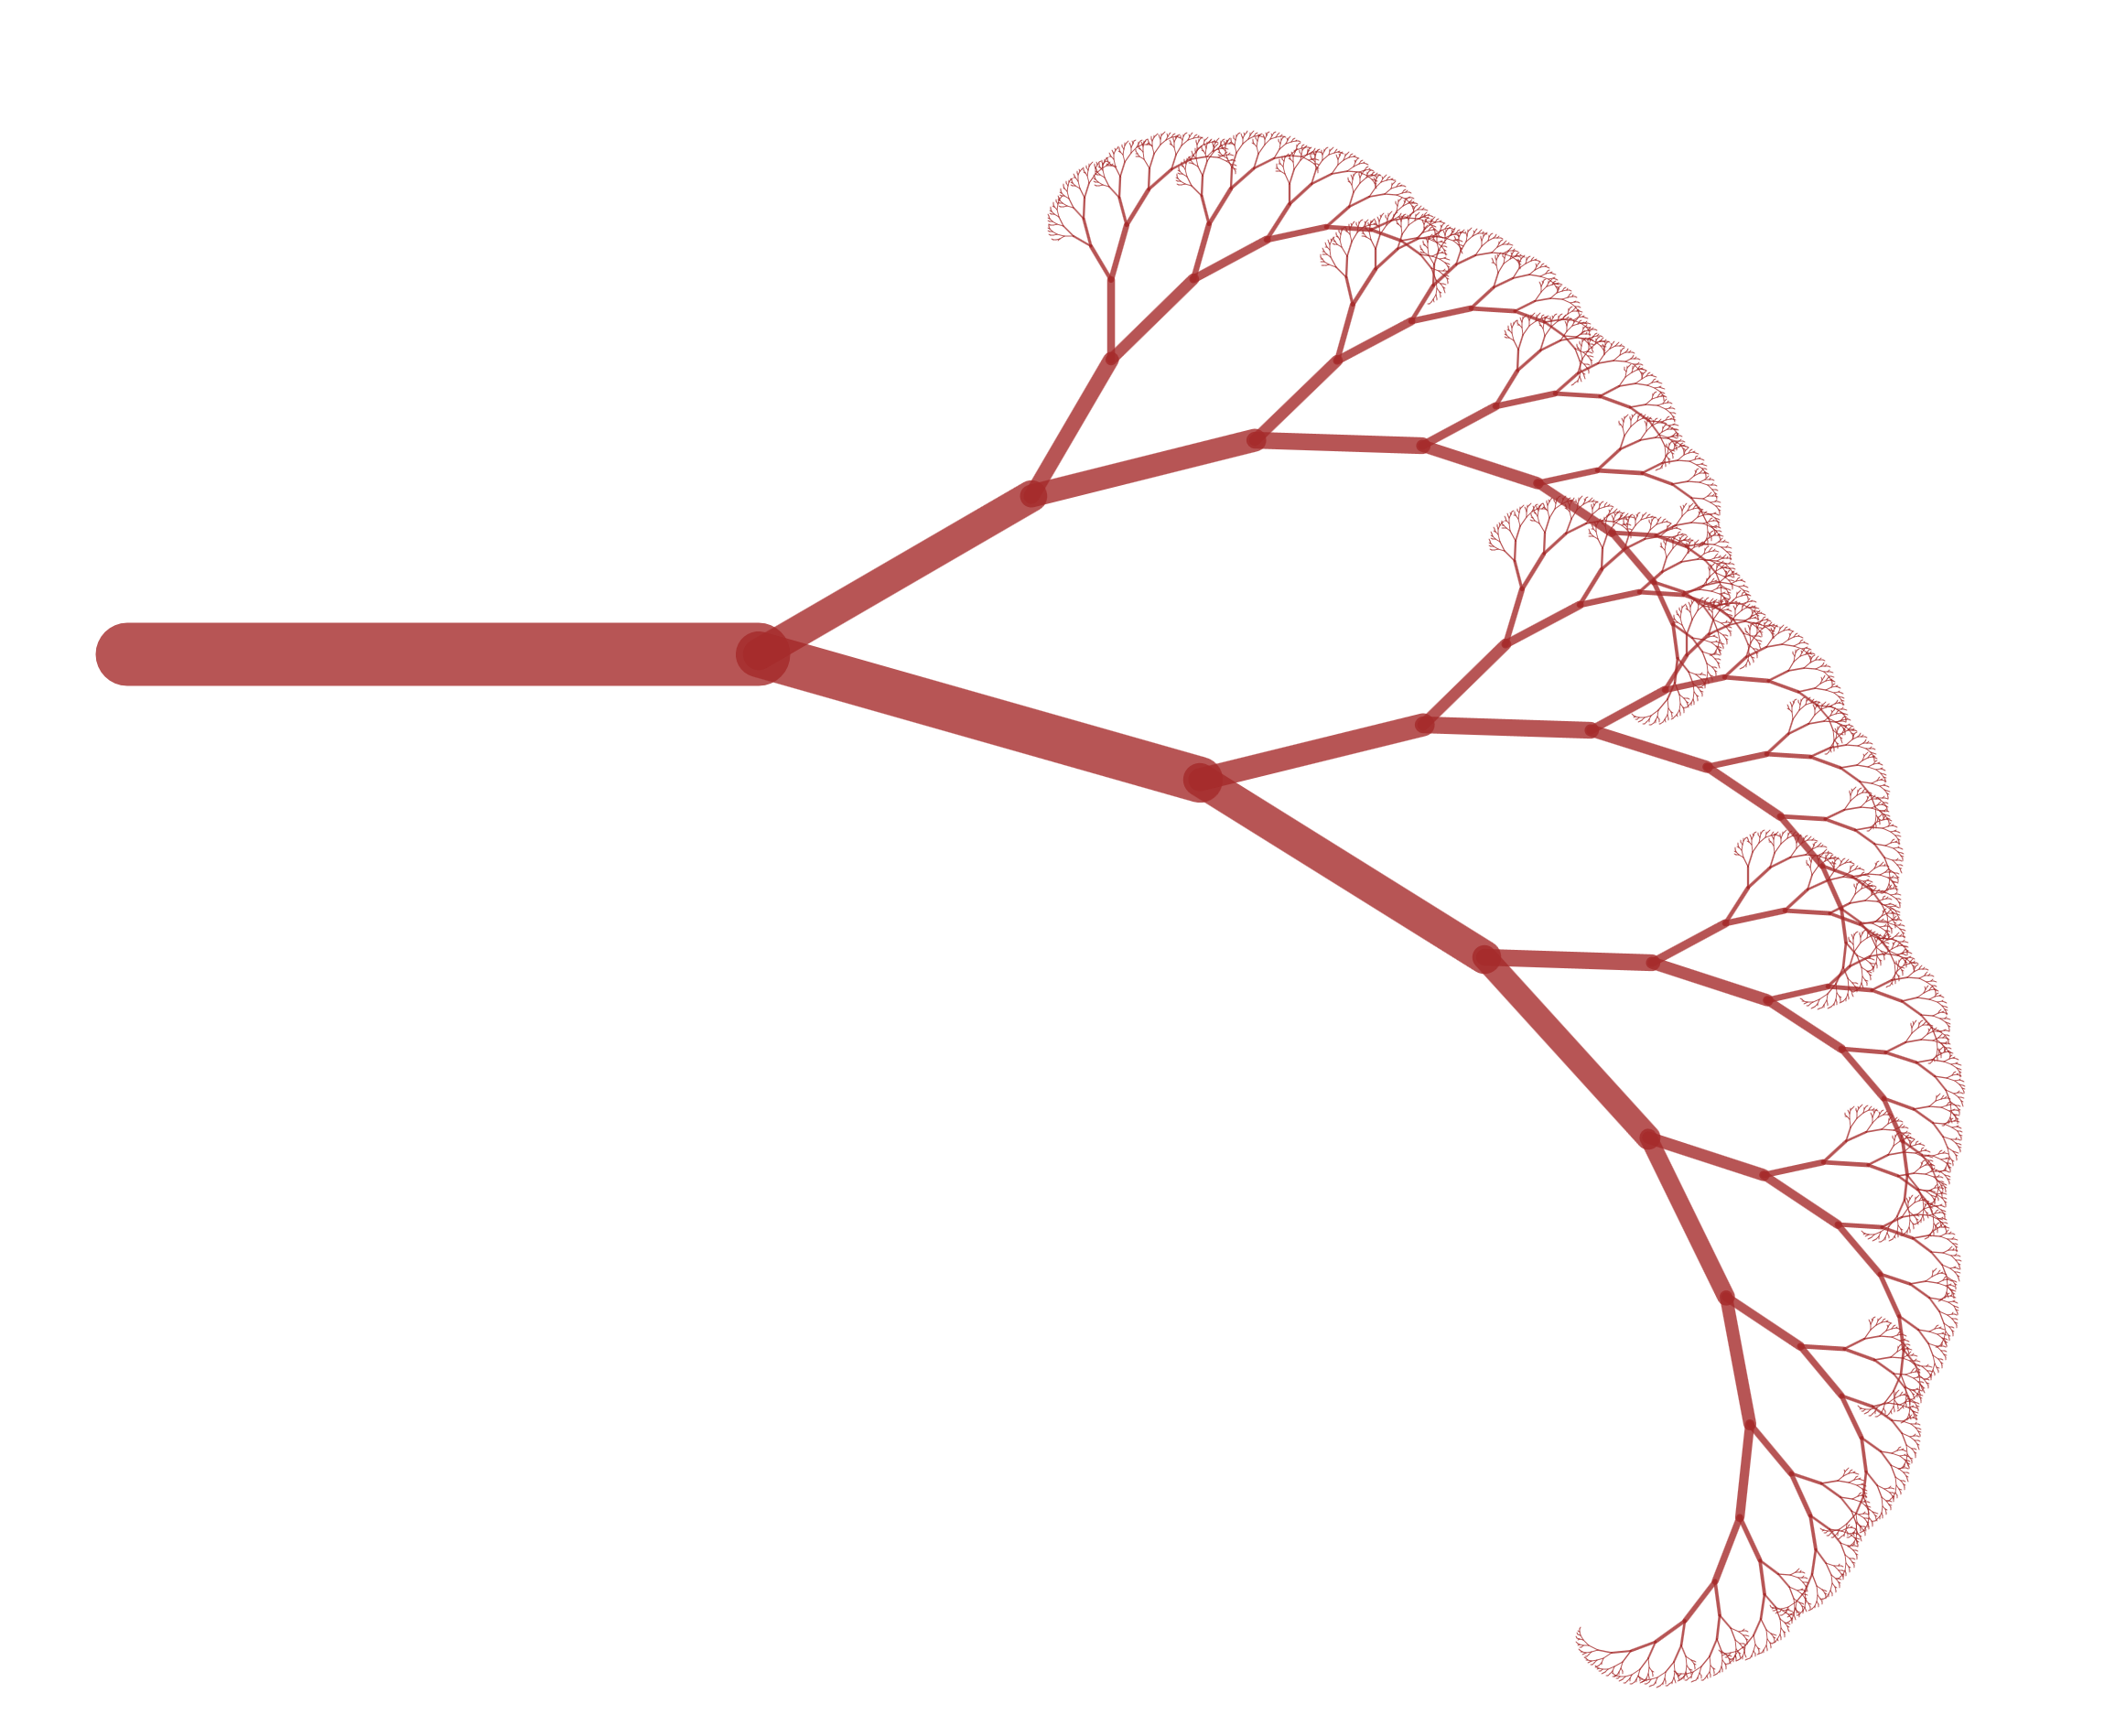
\includegraphics[width=0.8\textwidth]{img/simple03.png}
        \end{figure}

        \FloatBarrier

        Suppose then, that one would like to define several such functions, and combine them together.
        In order to accomplish that, there should be a way to tell apart different kinds of segments.
        A very straightforward method would be to give each segment a different color.
        In such a situation the previous example would translate to this (Figure~\ref{med01}).

        \begin{figure}[ht]
            \caption{\label{med01} Different Colors}
            \centering
            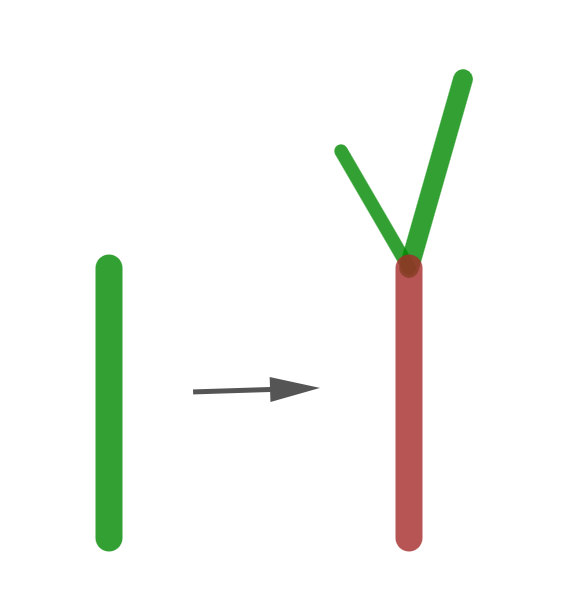
\includegraphics[width=0.16\textwidth]{img/med01.png}
        \end{figure}

        \FloatBarrier

        In this case the red segments will remain a simple segment while the green ones will transform further.
        Of course, it would be much clear if I would use arrows instead of simple segments because it might not be clear in which direction the segment should transform. 
        This will be discussed further in the paper.

        The fact that we use different colors allows not only to define a transformation in a much clear way, it also allows to implement much more interesting cases.
        Suppose that we have two functions defined in the following way.

        \begin{figure}[ht]
            \caption{\label{med02} Two transformation}
            \centering
            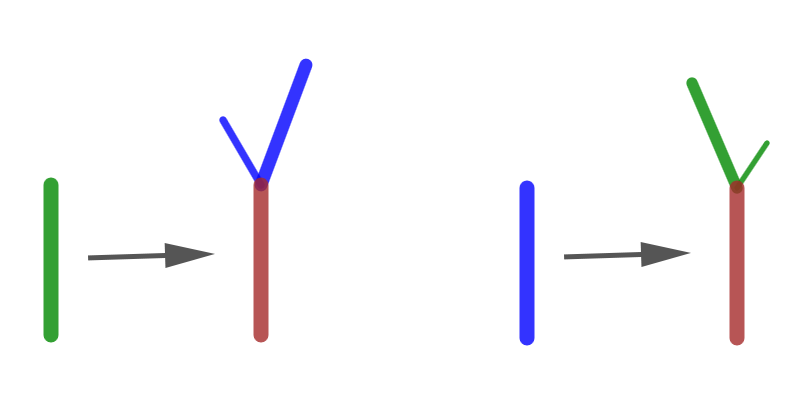
\includegraphics[width=0.4\textwidth]{img/med02.png}
        \end{figure}

        \FloatBarrier

        As one can see (Figure~\ref{med03}), this produces a fractal that is surprisingly similar to a real tree, even though the rules used are fairly simple.
        If we start with the blue segment instead of the green one, we get a slightly different tree, Figure~\ref{med04}.

        \begin{figure}[ht]
            \caption{\label{med03} A simple fractal tree.}
            \centering
            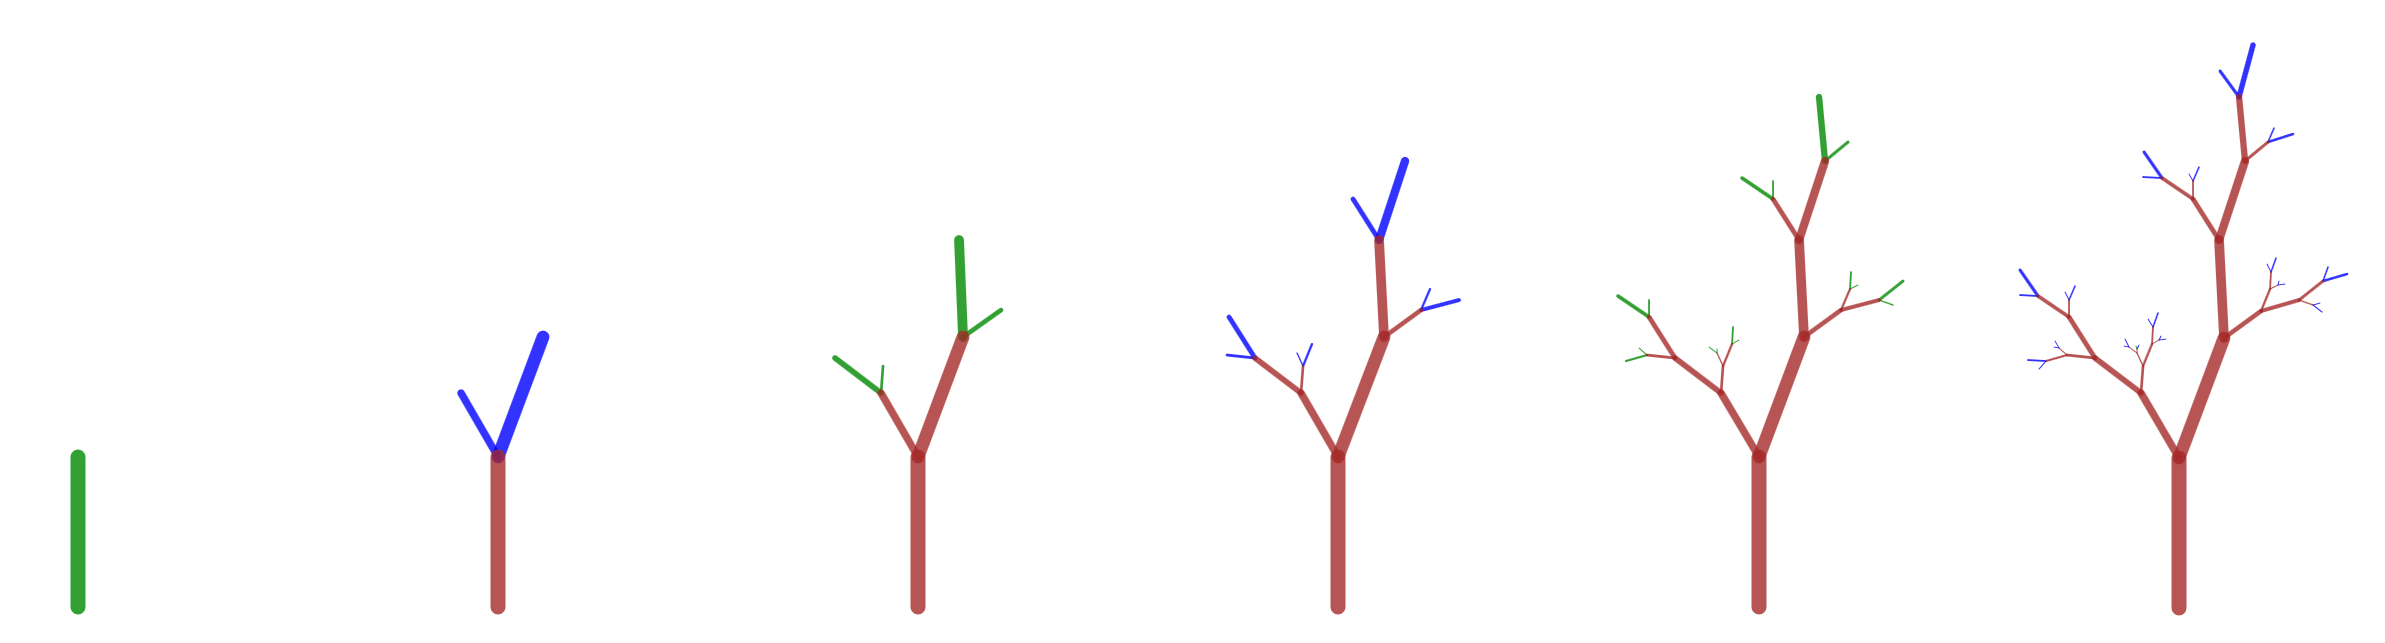
\includegraphics[width=0.9\textwidth]{img/med03.png}
        \end{figure}

        \begin{figure}[ht]
            \caption{\label{med04} Another simple fractal tree.}
            \centering
            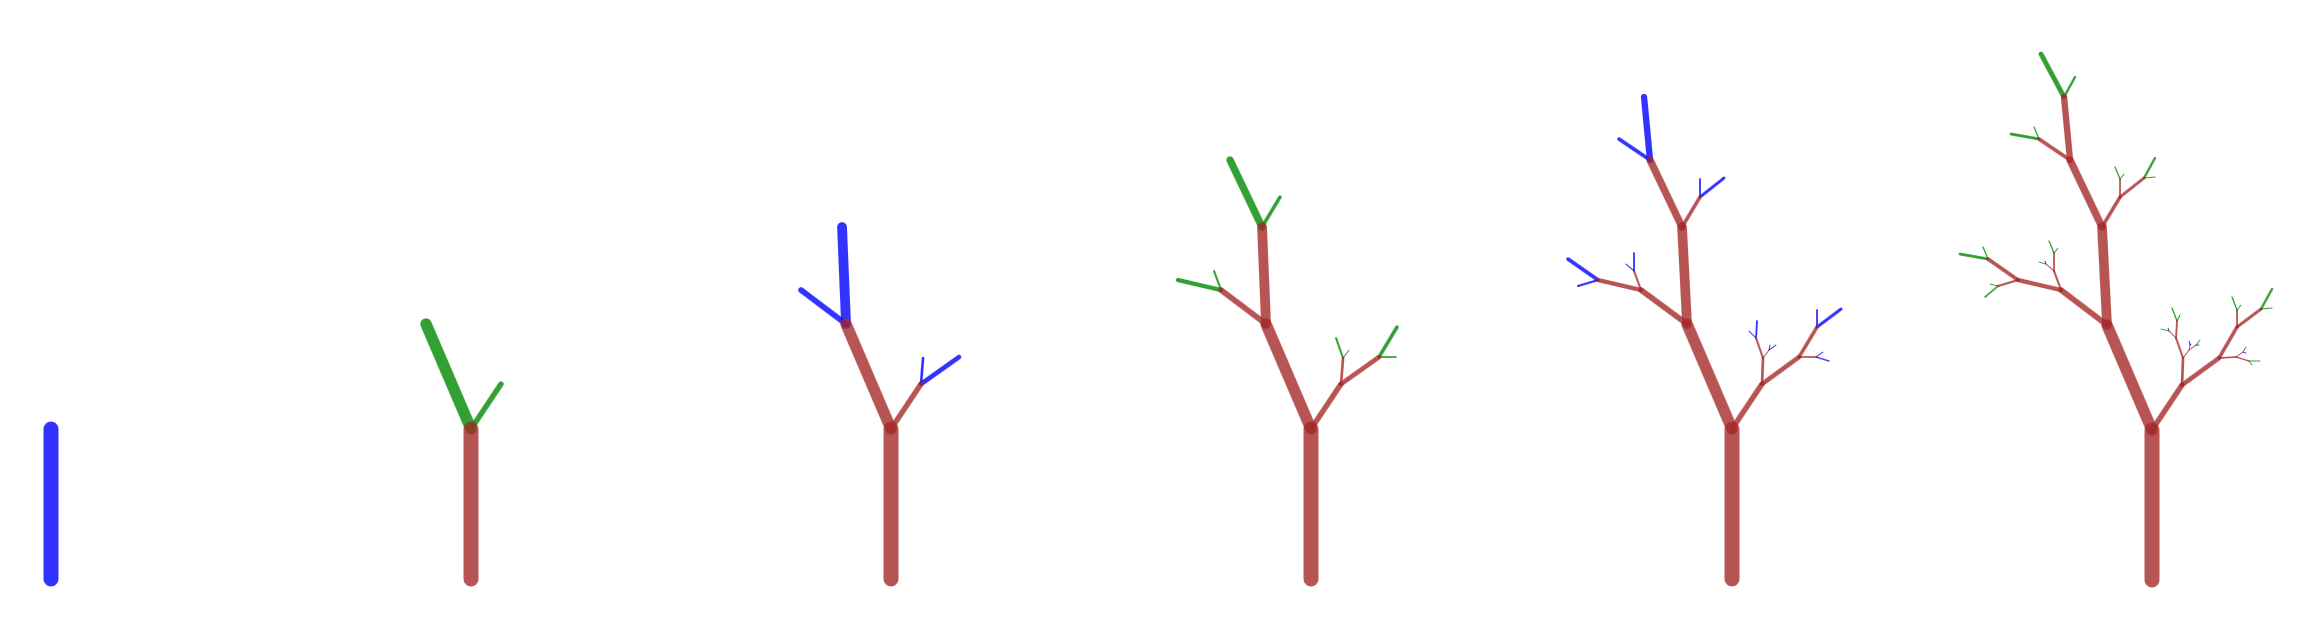
\includegraphics[width=0.9\textwidth]{img/med04.png}
        \end{figure}

        Figure~\ref{med05} shows the fractals in bigger detail.

        \begin{figure}[ht]
            \caption{\label{med05} Detailed Trees.}
            \centering
            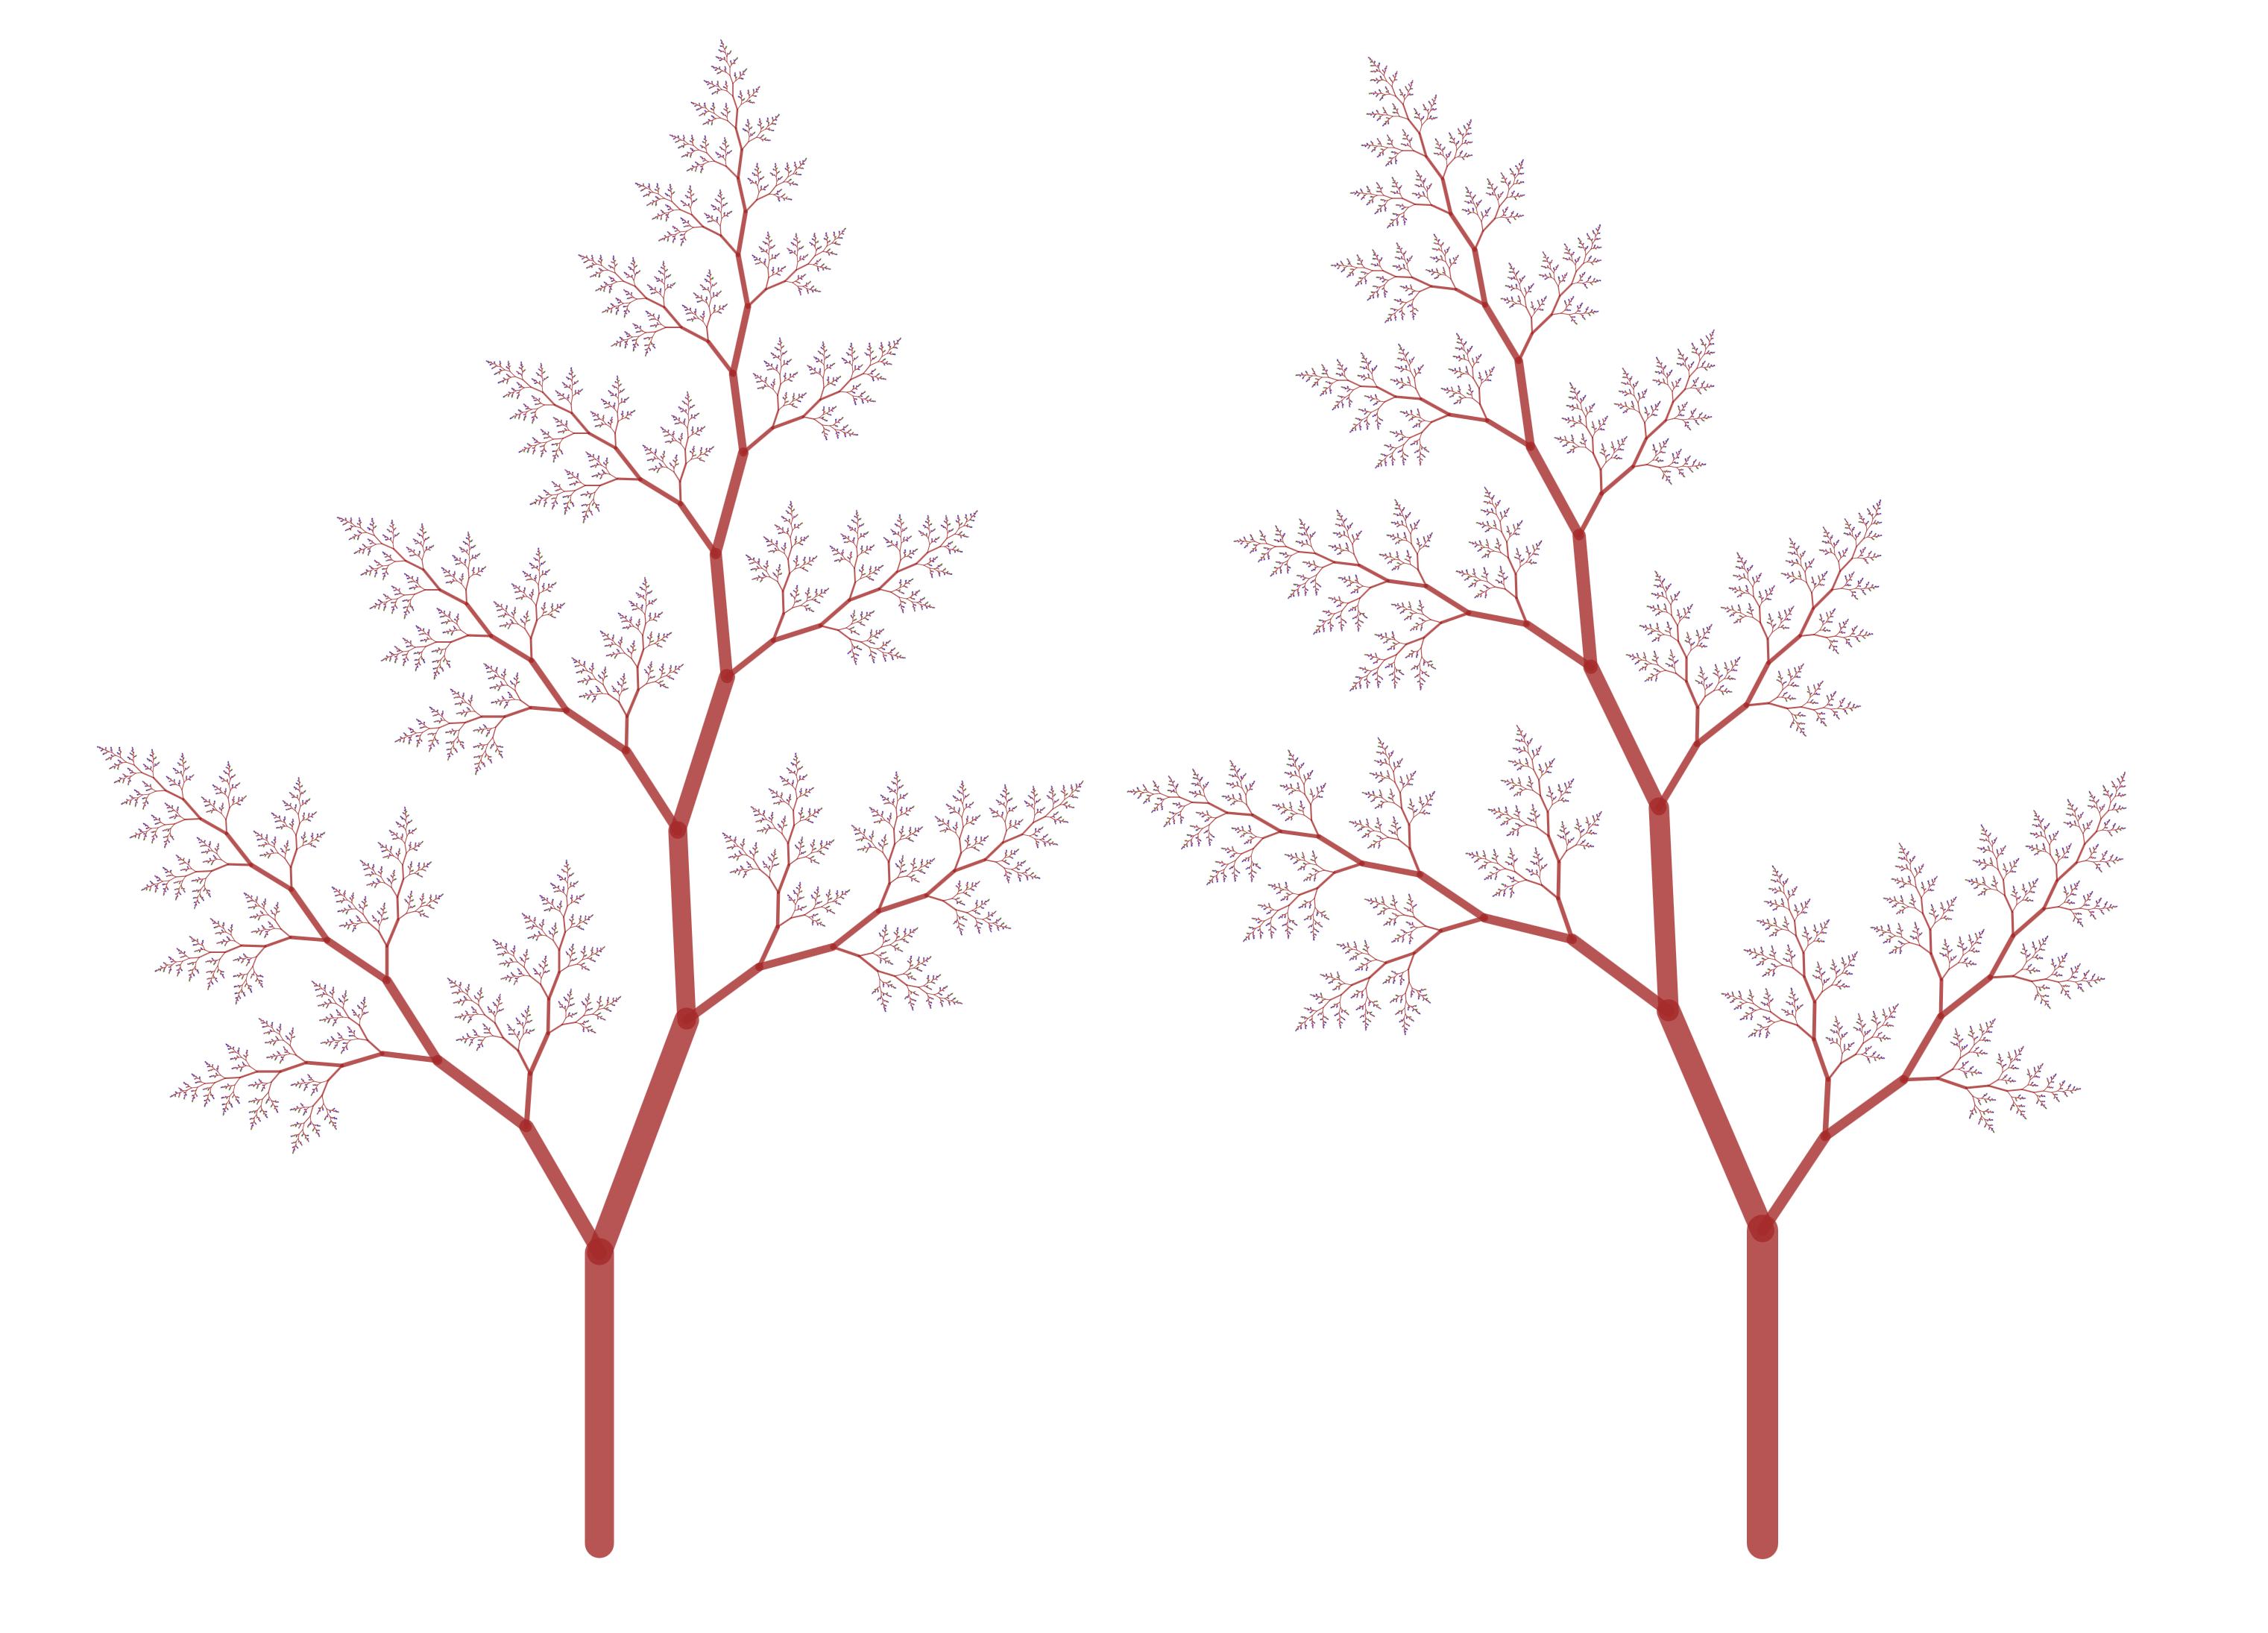
\includegraphics[width=\textwidth]{img/med05.png}
        \end{figure}

        \FloatBarrier

        At this moment, most of the readers might understand the basic idea of this project.
        In the next chapter I will try to explain how the GUI works and how the reader can create fractals by himself.

    \subsection{First steps}

        As I mentioned earlier, I started the work on the project with the idea that the program will be easy to use.
        There might exist other tools that allow the creation of iterated fractals, but most of them require advanced mathematical knowledge to understand and are a little cumbersome to use.

        \subsubsection{Basic controls}

            The way in which the user can create and manipulate a transformation is by dragging some circles.
            The circles can be dragged around by pressing and moving the \emph{left mouse button}.
            To create a new circle a user can press the \emph{right mouse button} on the background.
            To delete a circle the user should click the \emph{middle mouse button}.

            To create and arrow, one should drag a circle with the \emph{right mouse button}.
            To delete a segment, one should click the segment with the \emph{middle mouse button}.
            To change the type of the segment, one should click the segment with the \emph{left mouse button}.

            The concept are this: 
            \begin{enumerate}
                \item left button = move/change
                \item right button = create
                \item middle button = delete
            \end{enumerate}
            These were all the basic instructions. 
            Knowing how to use them is enough to create and edit a segment transformation.

        \subsubsection{The base layer and simple layers}

            A transformation can be create inside a layer. 
            A new layer can be create by pressing the \emph{Add Layer} button.
            Figure~\ref{gui01} shows how a new layer looks.

            \begin{figure}[ht]
                \caption{\label{gui01} A new layer.}
                \centering
                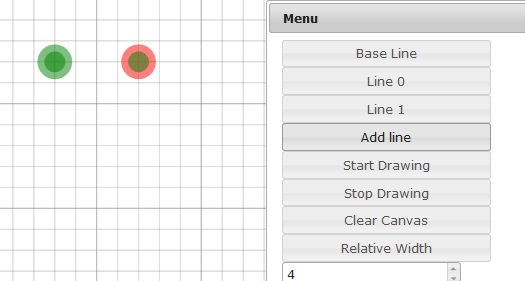
\includegraphics[width=0.5\textwidth]{img/gui01.png}
            \end{figure}

            The inner color of the circles represents the color of the transformation.
            The outer color represents the type of specific circles inside a layer.
            The circle with the outer color green is the start point and the circle with the outer color red is the end point.

            Lets try to implement the tree showed previously.
            First lets move the circles so that they stand vertically and also add two circles by pressing the \emph{right mouse button} on the background.

            \begin{figure}[ht]
                \centering
                \caption{Points and segments.}
                \subcaptionbox{\label{gui02} Two new points.}[.4\linewidth]
                    {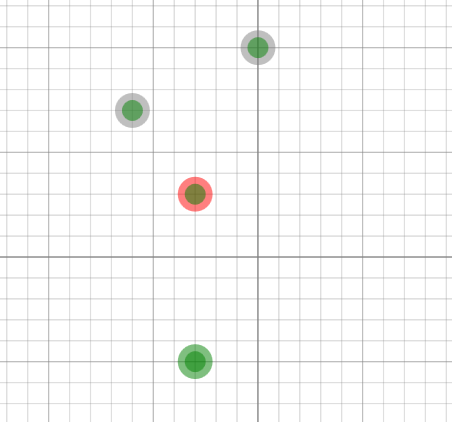
\includegraphics[height=0.35\textwidth]{img/gui02.png}}
                \subcaptionbox{\label{gui03} The first segments.}[.4\linewidth]
                    {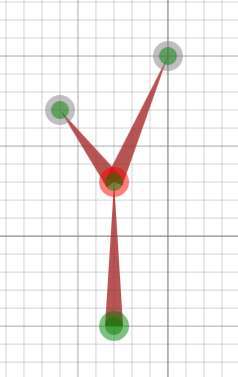
\includegraphics[height=0.35\textwidth]{img/gui03.png}}

            \end{figure}

            In order to create a segment the user should drag from a disk to another using the right mouse button (Figure~\ref{gui03}).

            \FloatBarrier

            It can be observed that all the arrows have the same color, red (it could be any other color). 
            But we didn't define a red type of transformation, so were do we have it.


        \subsubsection{Identity Layer}

            If we'll switch to Layer 0 by clicking the appropriate button we will see this (Fig.~\ref{identity01}).
            You can observe that the inner color of the circles is different, that's because we switched to a different layer.

            \begin{figure}[ht]
                \caption{\label{identity01} The identity layer.}
                \centering
                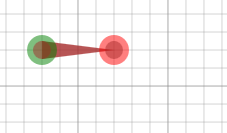
\includegraphics[width=0.3\textwidth]{img/identity01.png}
            \end{figure}

            The identity layer is a little bit different from other layers.
            First of all, even though we can drag the circles around, we cannot add more circles or change the type of the arrow.

            \FloatBarrier

            The identity layer draws itself, that is, it does not transform to something different.
            Because of this property, there are some optimizations that can be implemented.
            For example instead of recursing further when finding a identity layer, the program will just draw the line because it can infer that 
            the segment will not transform to something different.

            Coming back to Layer 1, we can click each of the upper arrows in order to change their colors (Fig.~\ref{gui04}).

            \begin{figure}[ht]
                \caption{\label{gui04} Different types of arrows.}
                \centering
                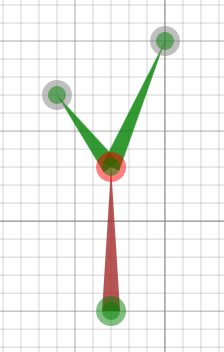
\includegraphics[width=0.2\textwidth]{img/gui04.png}
            \end{figure}
            \FloatBarrier

            The new color is green, that is, the color of the current layer.
            If we would click the arrows one more time they would, once again, change their color to the color of the identity layer.

            Even though we basically define all that is required we don't see anything happening.

        \subsubsection{The Base Layer}

            The uppermost Layer (Fig.~\ref{baselayer01}), called the base layer is different from all the other layers.
            First of all it does not have a initial green and red circle. 

            \begin{figure}[ht]
                \caption{\label{baselayer01} The Base Layer.}
                \centering
                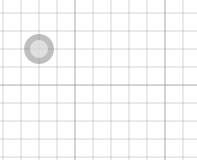
\includegraphics[width=0.2\textwidth]{img/baselayer01.png}
            \end{figure}

            The base layer is used not to define a transformation but to apply them.
            Lets create another point and connect these two points with an arrow.

            \begin{figure}[H]
                \centering
                \caption{Changing the color of the arrow.}
                \subcaptionbox{\label{baselayer02} First try.}[0.4\textwidth]
                    {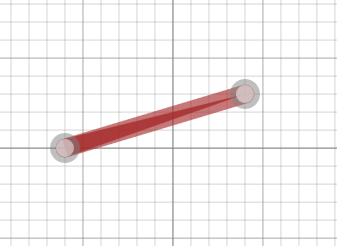
\includegraphics[width=0.3\textwidth]{img/baselayer02.png}}
                ~
                \subcaptionbox{\label{baselayer03} Second try.}[0.5\textwidth]
                    {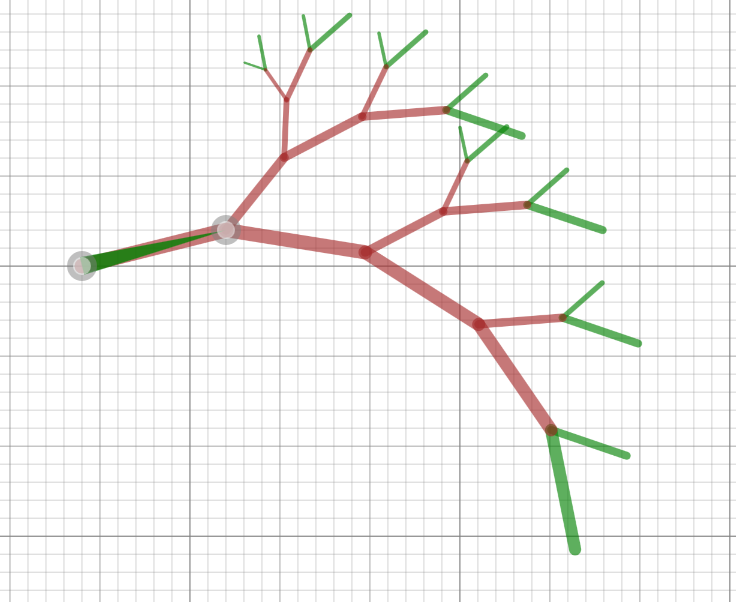
\includegraphics[width=0.45\textwidth]{img/baselayer03.png}}
            \end{figure}

            Something interesting happens. 
            Just as we connected the circles, an thick arrow appeared on the background.
            Because the arrow is of identity type it just created a line.
            Lets try to press the arrow in order to change the type.

            \FloatBarrier

            Figure~\ref{baselayer03} shows that we created our first, own fractal tree.
            If we move the circles around the tree will move along.
            This is because the \emph{Dynamic Drawing} check-box is on, we'll talk about this feature later.

            Another interesting feature is that if we switch to Layer 1 and move the circles there, the tree will also change (Fig.~\ref{baselayer04}).
            It is important to not get confused at this point.
            For some it might be strange that the the root of the tree does not coincide with the identity arrow in Layer 1.
            This is because Layer are used to define transformation that are applied to the Base Layer.
            Only the Base Layer defines the position of the initial segments.

            \begin{figure}[ht]
                \caption{\label{baselayer04} Perspective from another layer.}
                \centering
                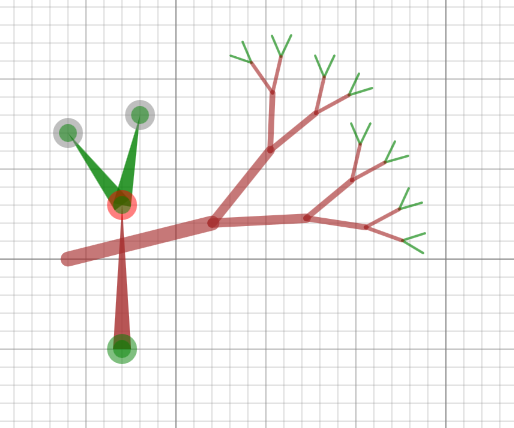
\includegraphics[width=0.3\textwidth]{img/baselayer04.png}
            \end{figure}

    \subsection{Common fractals}

        During this and the subsequent chapters I will show some fractals and other geometric structures that can be created using this soft.
        Also, in this way I will try to give some insight and useful information about the GUI.
        I think that a hands-on approach would be much more insightful than any other method of explanation.

        \subsubsection{The Dragon Curve}

            The Dragon Curve is very easy to create.
            This setup (Fig.~\ref{dragon01}) is required in a new layer.

            \begin{figure}[ht]
                \caption{The Dragon Curve.}
                \centering
                \subcaptionbox{\label{dragon01} The setup.}[0.3\textwidth]
                    {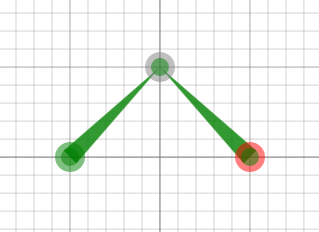
\includegraphics[width=0.3\textwidth]{img/dragon01.png}}
                ~
                \subcaptionbox{\label{dragon02} Dragon Curve after 4 steps.}[0.3\textwidth]
                    {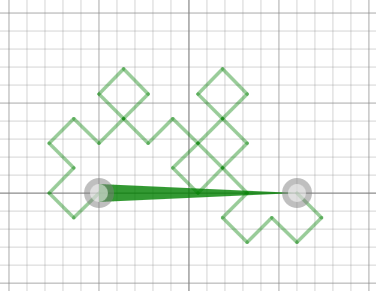
\includegraphics[width=0.3\textwidth]{img/dragon02.png}}
            \end{figure}

            Adding a arrow in the base layer we get this (Fig.~\ref{dragon02}).

            To increase the recursion level the user must use the spinner in the main dialog.
            This is what can be created (Fig.~\ref{dragon03}).

            \begin{figure}[ht]
                \caption{\label{dragon03} The Dragon Curve.}
                \centering
                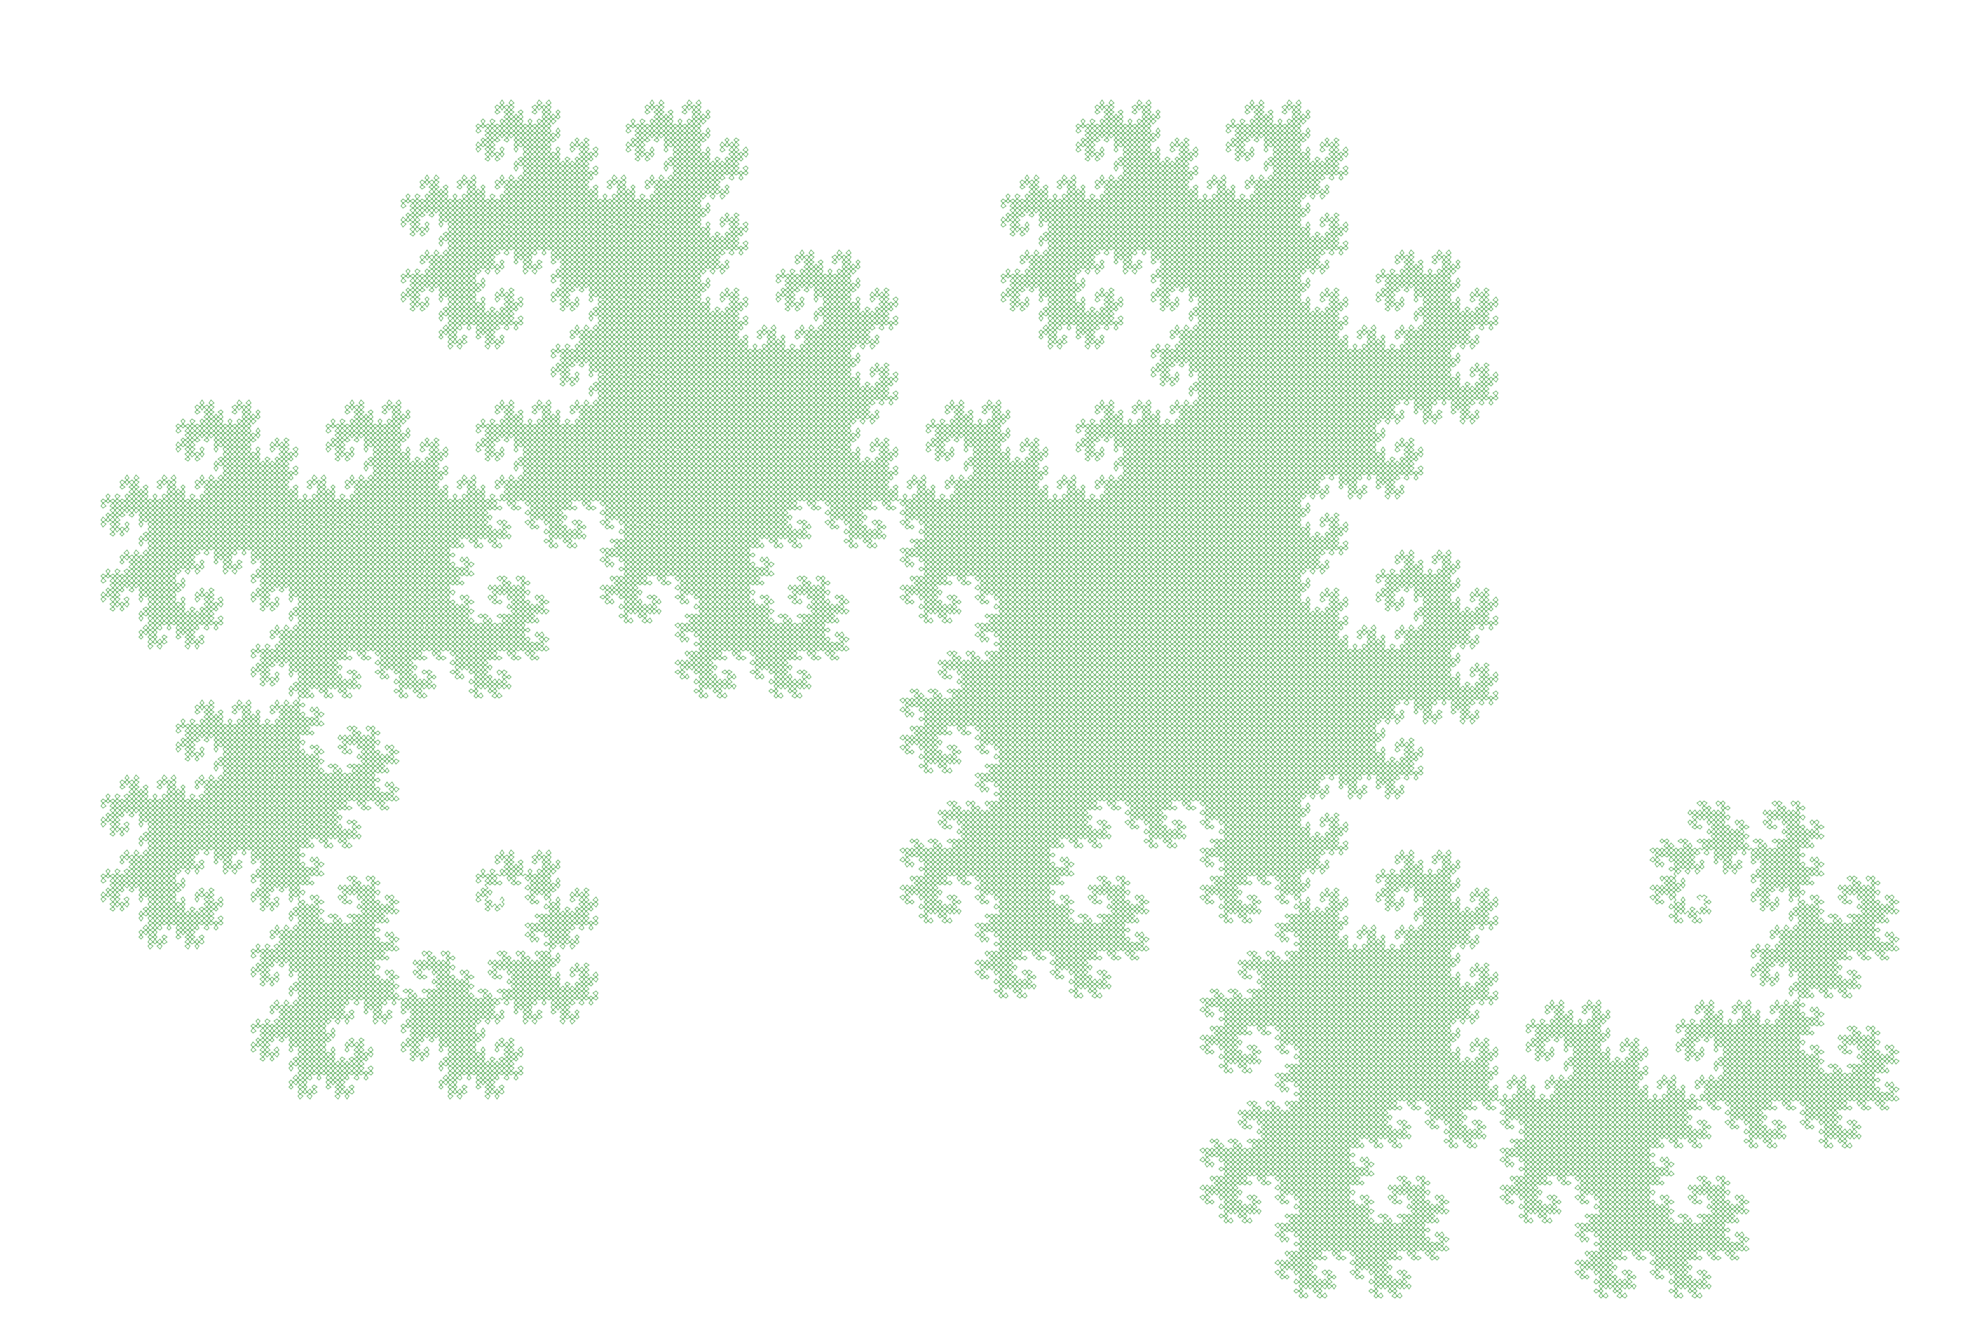
\includegraphics[width=0.96\textwidth]{img/dragon03.png}
            \end{figure}

            \FloatBarrier

        \subsubsection{Levy C Curve}

            The setup for the Levy C Curve is very similar to the Dragon Curve.
            
            \begin{figure}[ht]
                \caption{\label{levyc01} The setup.}
                \centering
                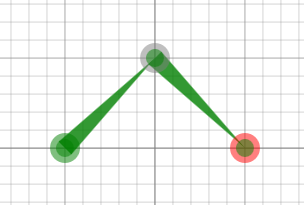
\includegraphics[width=0.3\textwidth]{img/levyc01.png}
            \end{figure}

            It is interesting that changing the direction of the arrow can have such an impact.

            \begin{figure}[ht]
                \caption{\label{levyc02} Levy C Curve.}
                \centering
                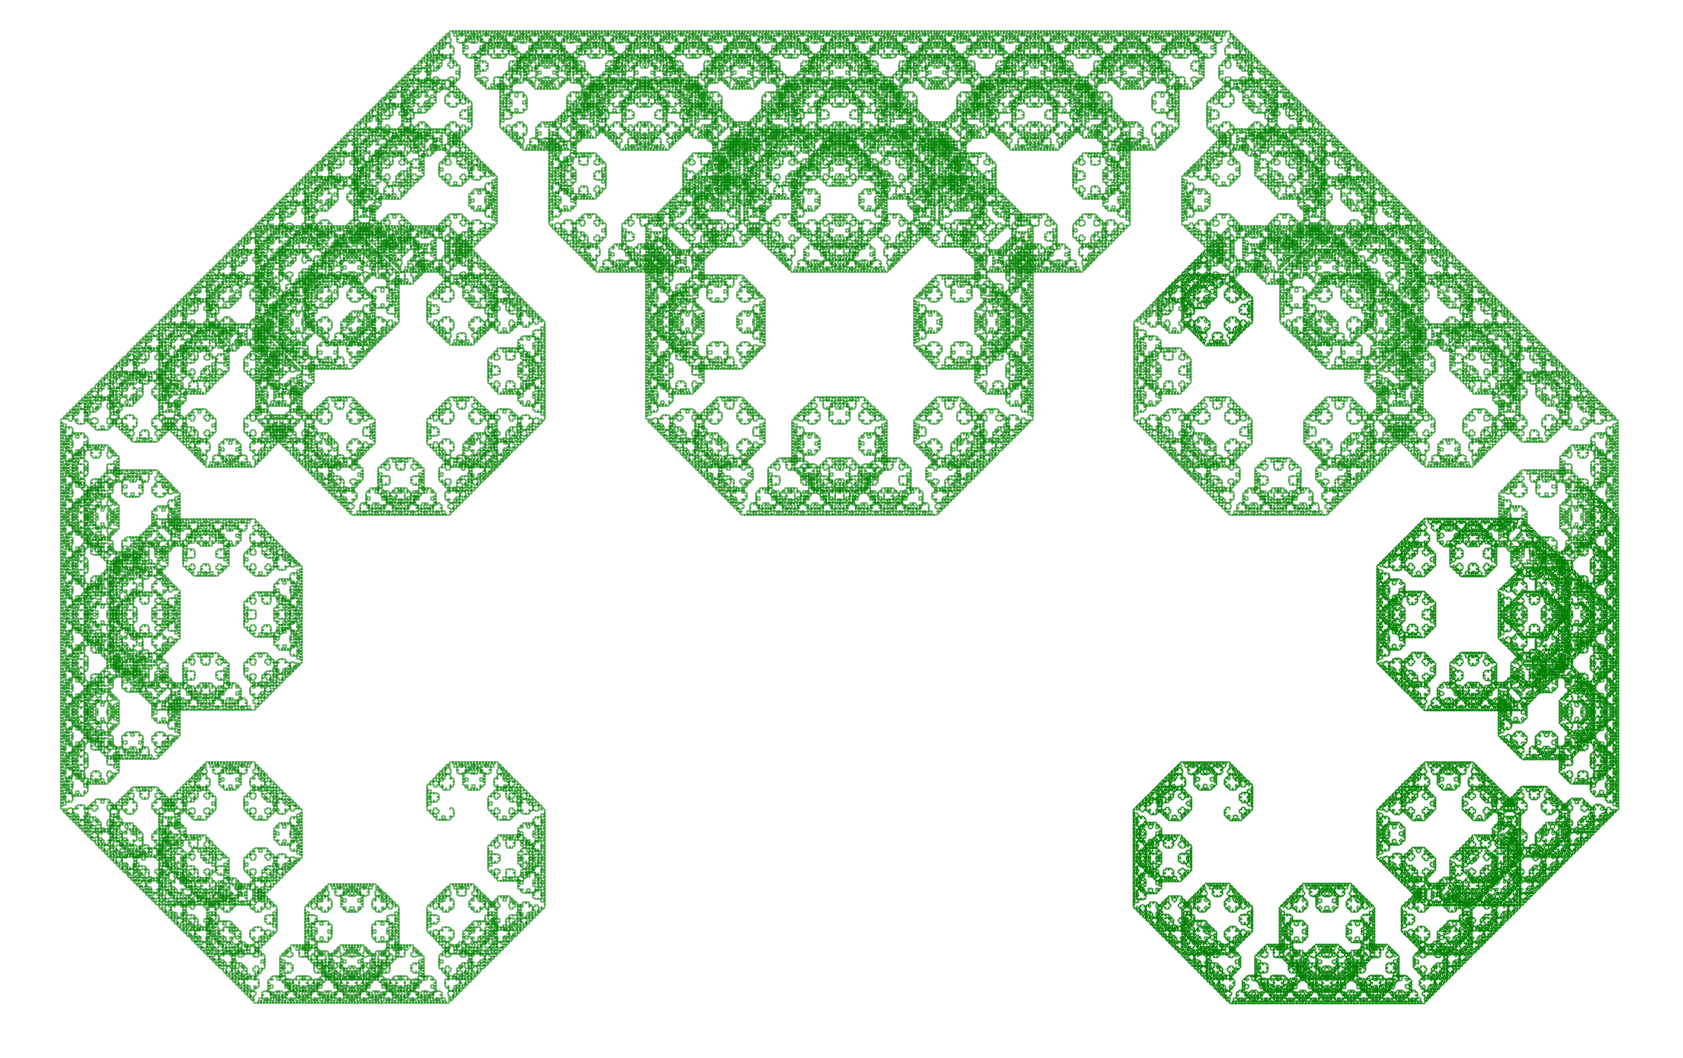
\includegraphics[width=0.9\textwidth]{img/levyc02.png}
            \end{figure}

            \FloatBarrier

        \subsubsection{Koch Snowflake and the Polar Grid}

            Lets try to create the Koch Snowflake.

            \begin{figure}[ht]
                \caption{Koch Snowflake.}
                \centering
                \begin{subfigure}[b]{0.49\textwidth}
                    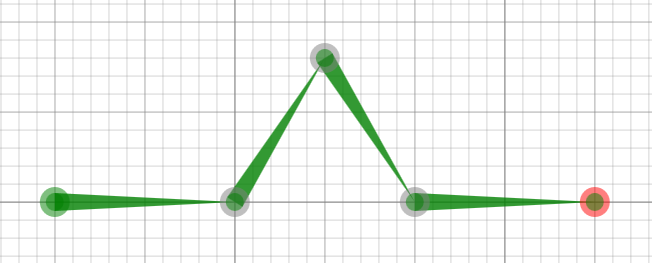
\includegraphics[width=\textwidth]{img/snowflake_setup.png}
                    \caption{Cartesian grid \label{snowflake_setup}}
                \end{subfigure}
                ~
                \begin{subfigure}[b]{0.49\textwidth}
                    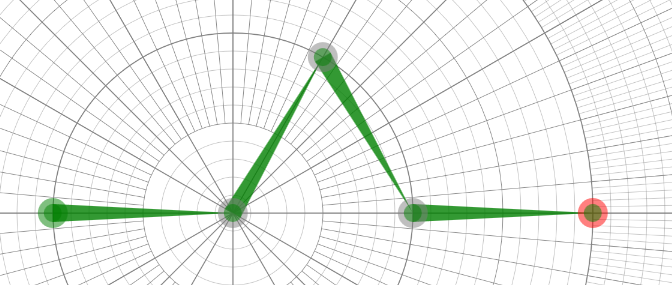
\includegraphics[width=\textwidth]{img/snowflake_setup02.png}
                    \caption{Polar grid \label{snowflake_setup_02}}
                \end{subfigure}
            \end{figure}

            The problem, as one can see, is that it is basically impossible to create an angle of 60 degrees using the cartesian coordinates.
            To solve this problem I came up with an interesting idea.
            I implemented a polar grid.
            To switch to it the user has to press the \emph{Polar Grid} button.
            The center of the polar grid will be \emph{the last pressed circle}.
            Below is the new setup.

            The setup in the Base Layer can be the following (Fig.~\ref{snowflake_setup03}).

            \begin{figure}[ht]
                \caption{\label{snowflake_setup03} Base Layer setup.}
                \centering
                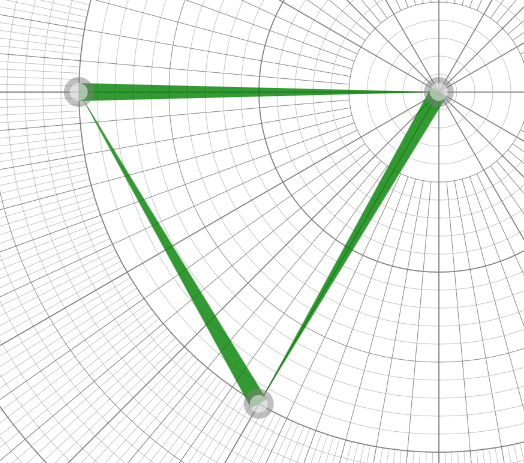
\includegraphics[width=0.3\textwidth]{img/snowflake_setup03.png}
            \end{figure}

            The drawing is in Figure~\ref{snowflake_draw}.

            \begin{figure}[ht]
                \caption{\label{snowflake_draw} Koch Snowflake.}
                \centering
                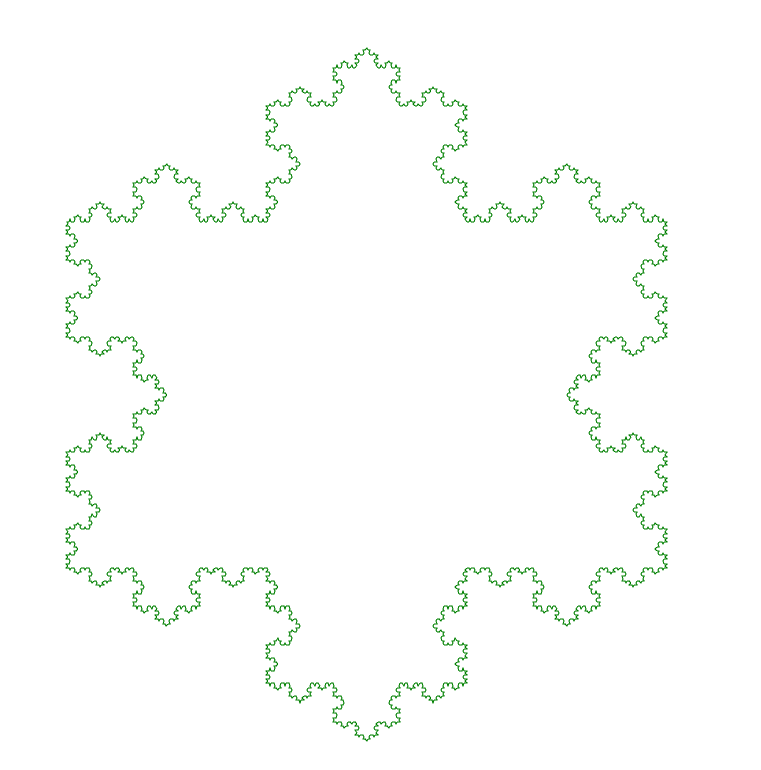
\includegraphics[width=0.6\textwidth]{img/snowflake_draw.png}
            \end{figure}

            \FloatBarrier

        \subsubsection{Some Quadratic curves}

            Following Koch's concept other types of curves were introduced.

            \begin{figure}[ht]
                \caption{\label{quadratic_01} Quadratic type 1.}
                \centering
                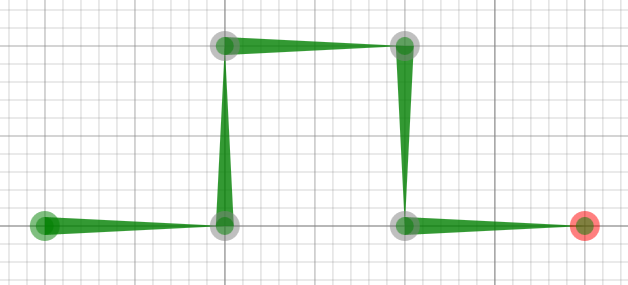
\includegraphics[width=0.3\textwidth]{img/quadratic_01setup.png}
                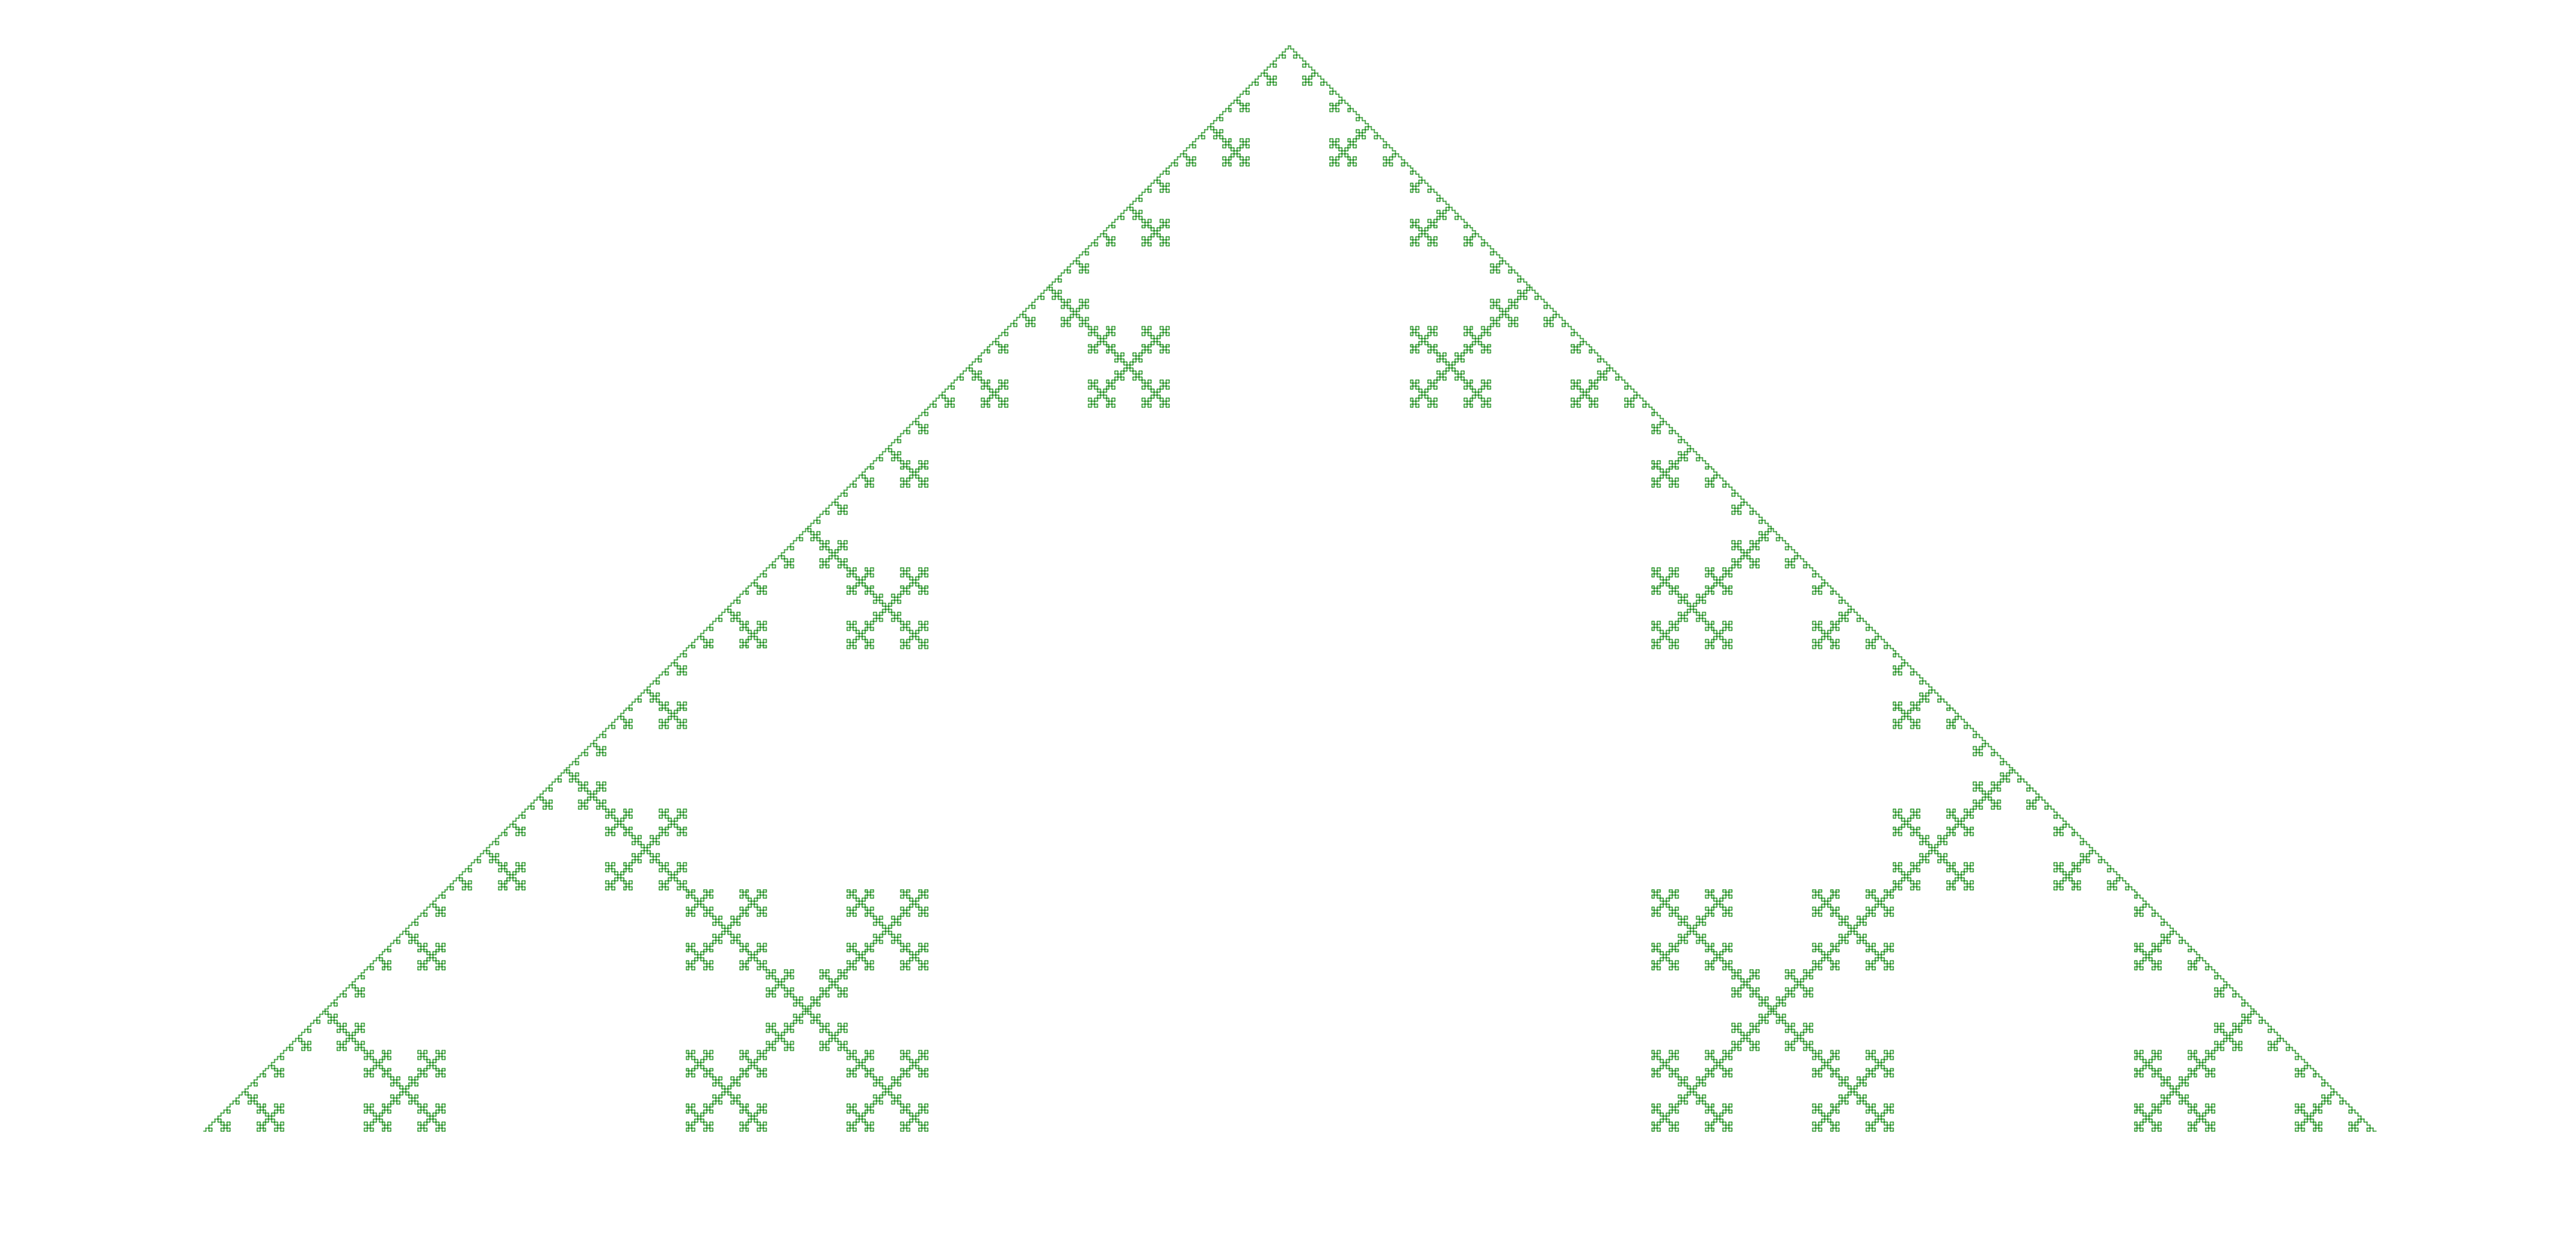
\includegraphics[width=0.67\textwidth]{img/quadratic_01draw.png}
            \end{figure}

            \begin{figure}[ht]
                \caption{\label{quadratic_02} Quadratic type 2.}
                \centering
                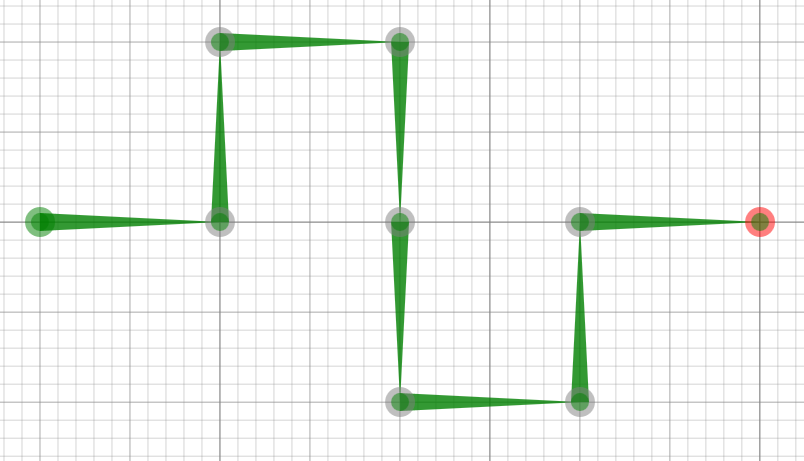
\includegraphics[width=0.3\textwidth]{img/quadratic_02setup.png}
                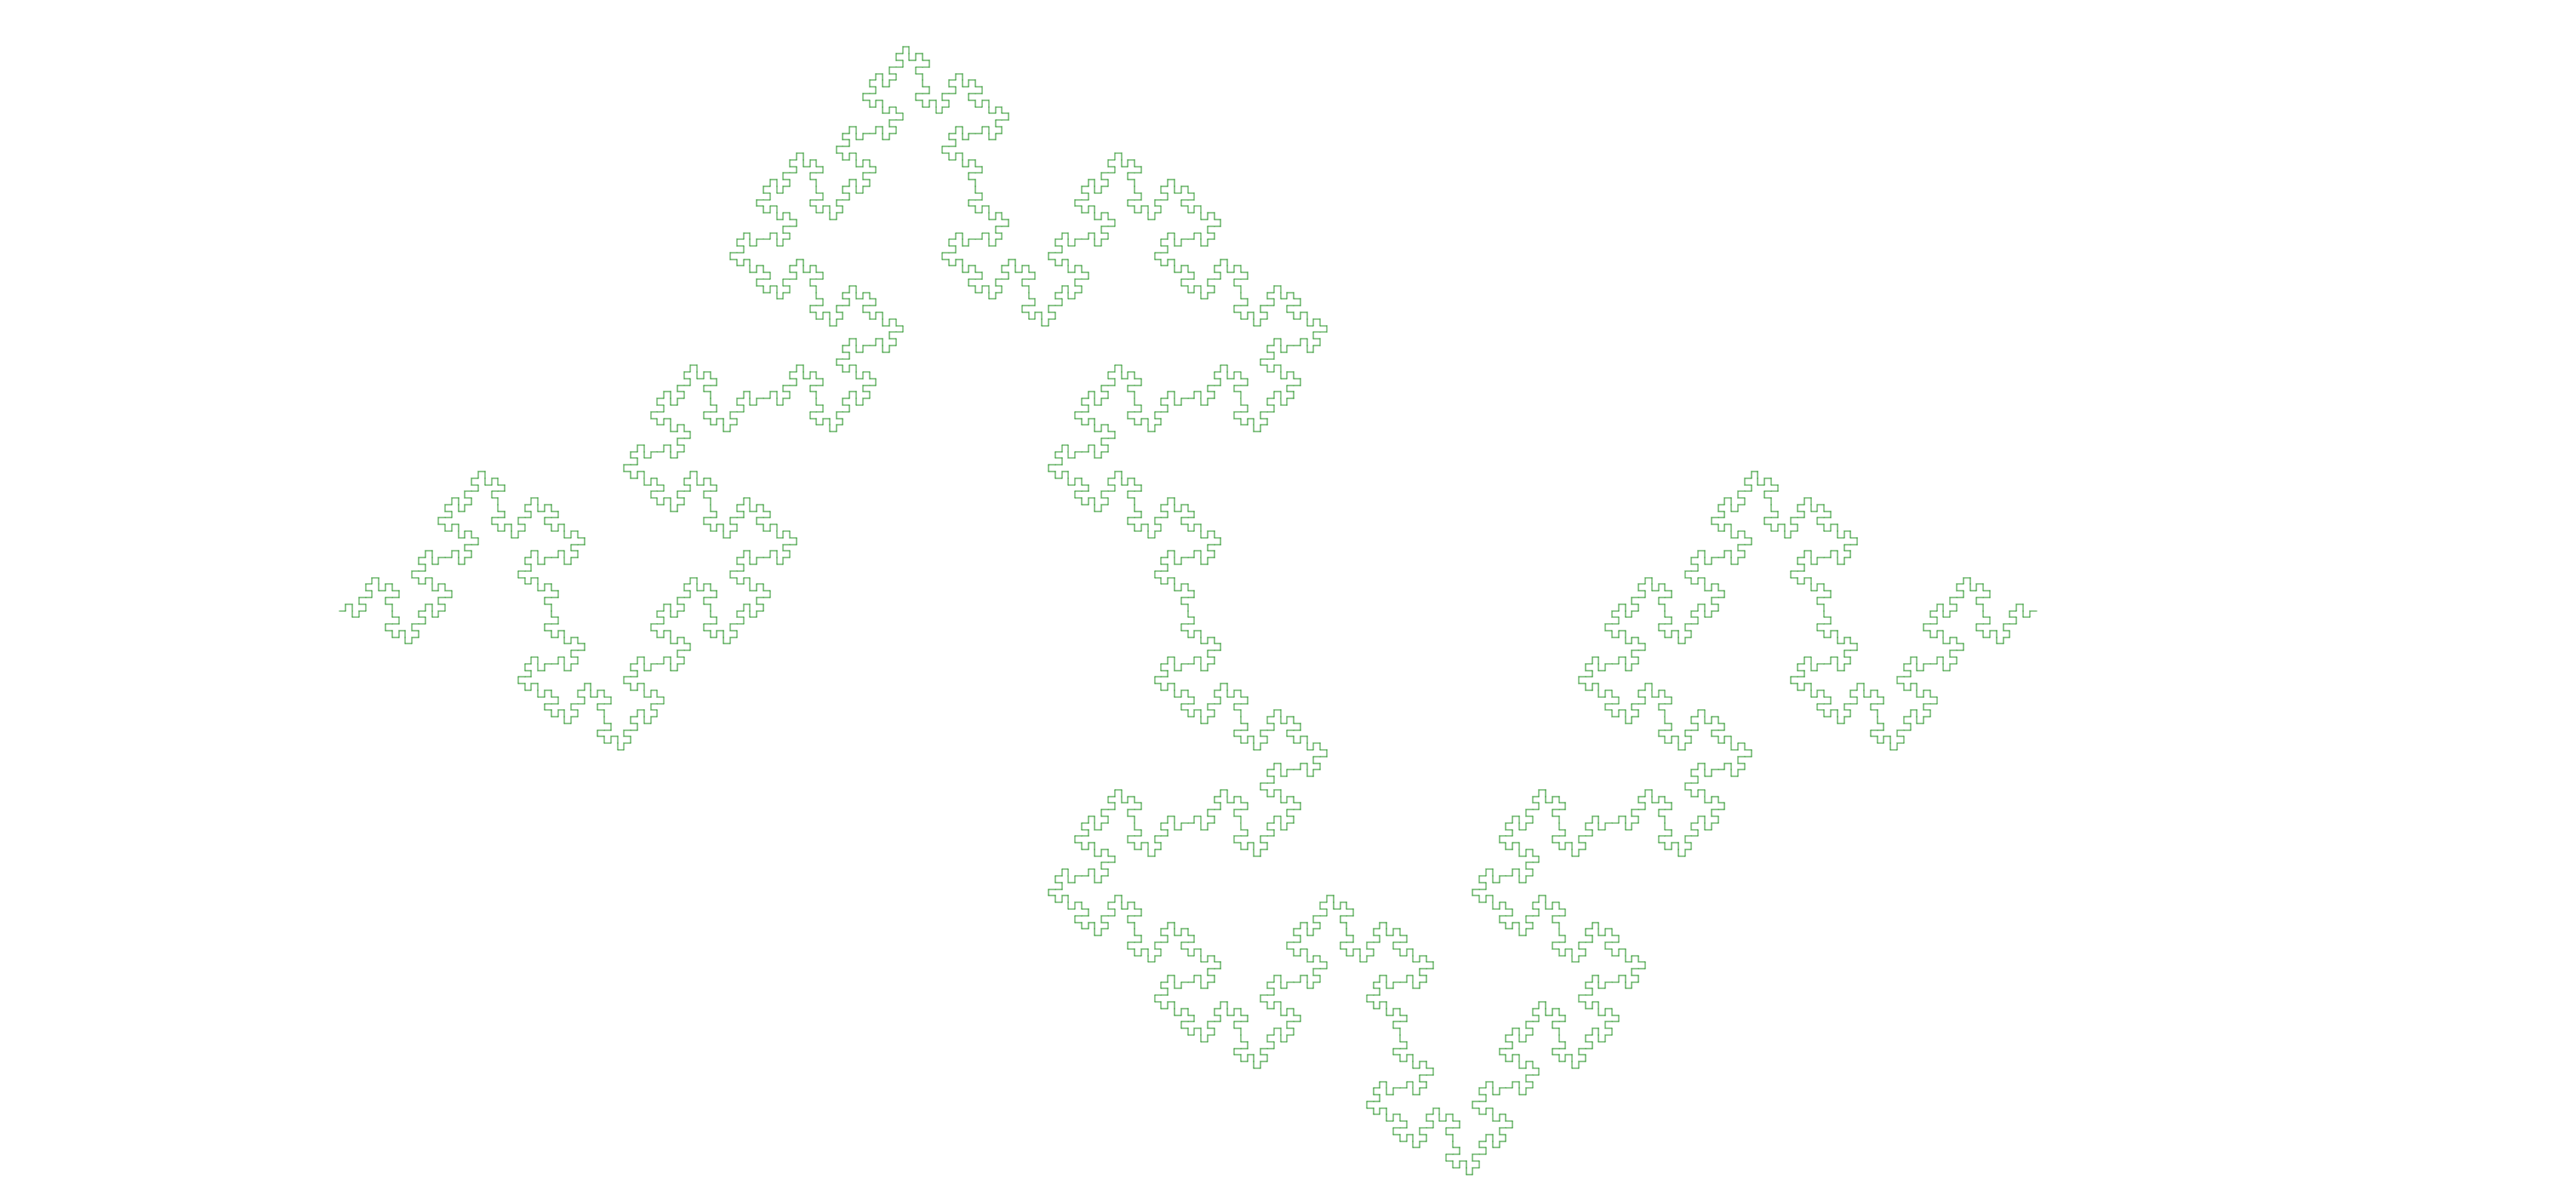
\includegraphics[width=0.67\textwidth]{img/quadratic_02draw.png}
            \end{figure}

            \FloatBarrier

        \subsubsection{Variations}

            At this moment it will probably be already clear that the program is not bound to create rigorously defined fractals. 
            The user can choose to create a lot of different variations with ease.
            The fact that the lines are drawn dynamically make this even more interesting.
            The pictures in Figure \ref{koch_variatinos_01} show just a very few of the types of Koch curve variations that can be created.
            I will come back to Koch variations in later chapter.

            \begin{figure}[ht]
                \caption{\label{koch_variatinos_01} Koch Curve variations}
                \centering
                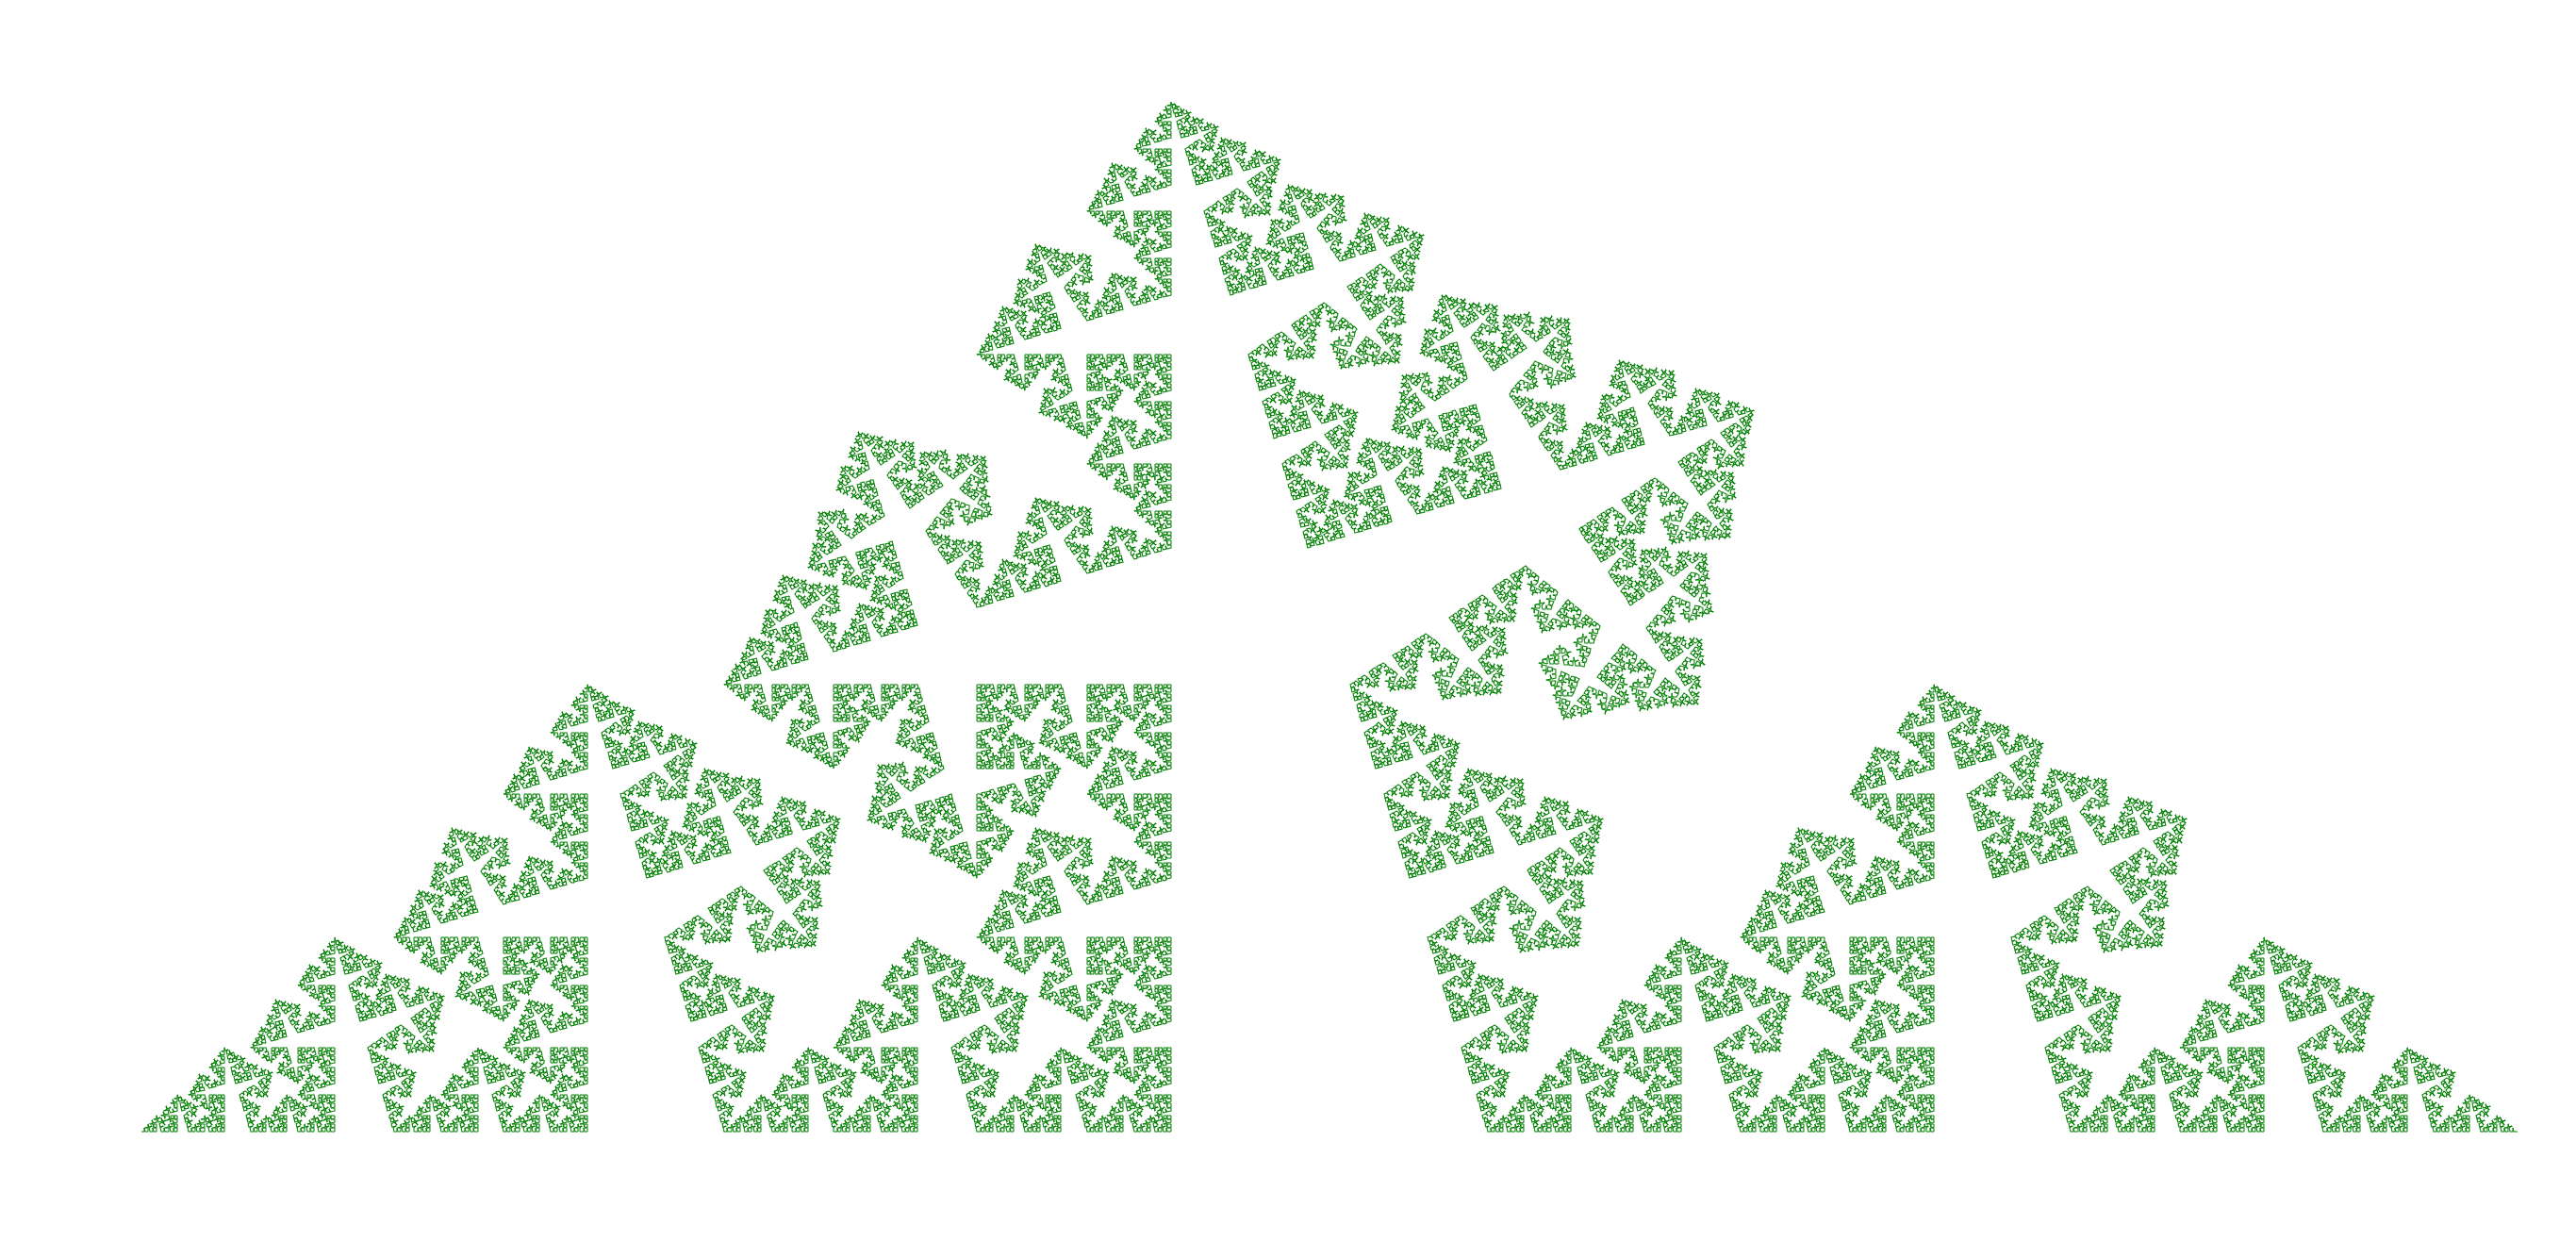
\includegraphics[width=0.49\textwidth]{img/Simple_Variations/koch_variation_01.png}
                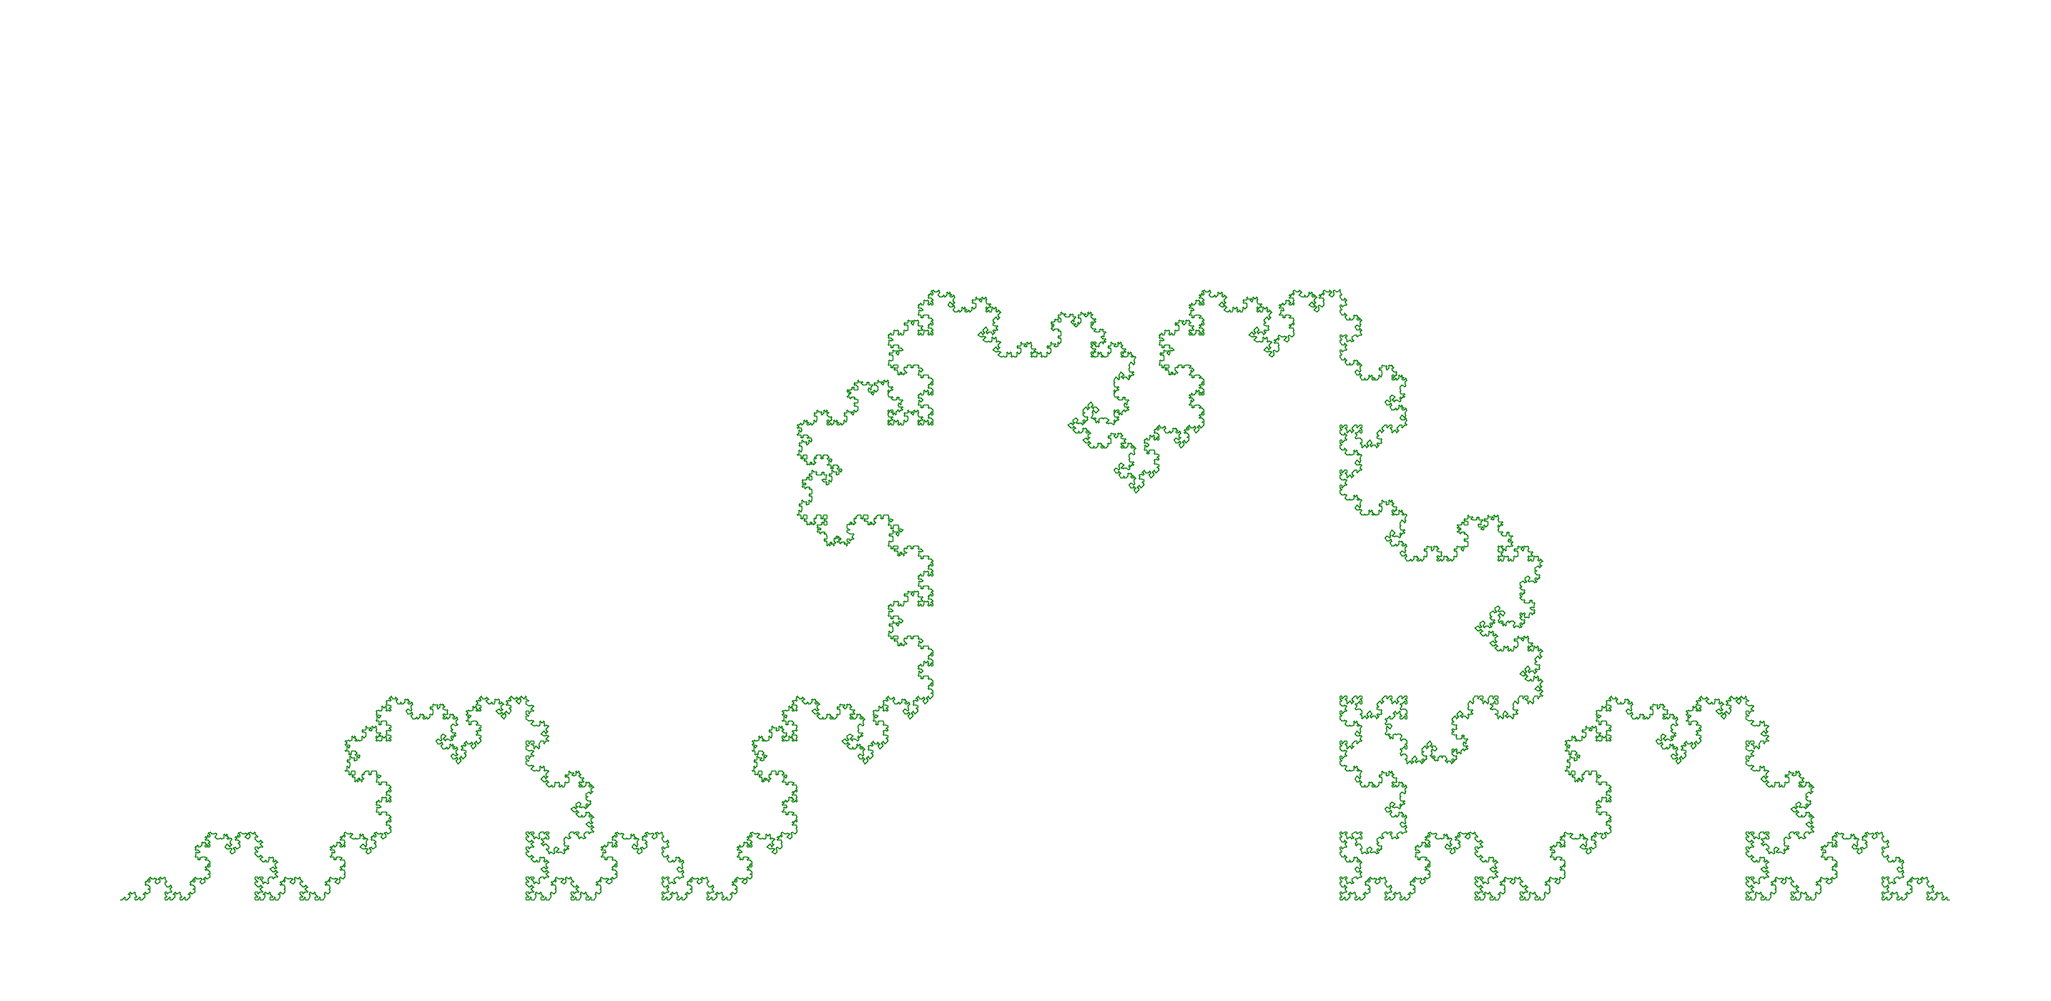
\includegraphics[width=0.49\textwidth]{img/Simple_Variations/koch_variation_02.png}
                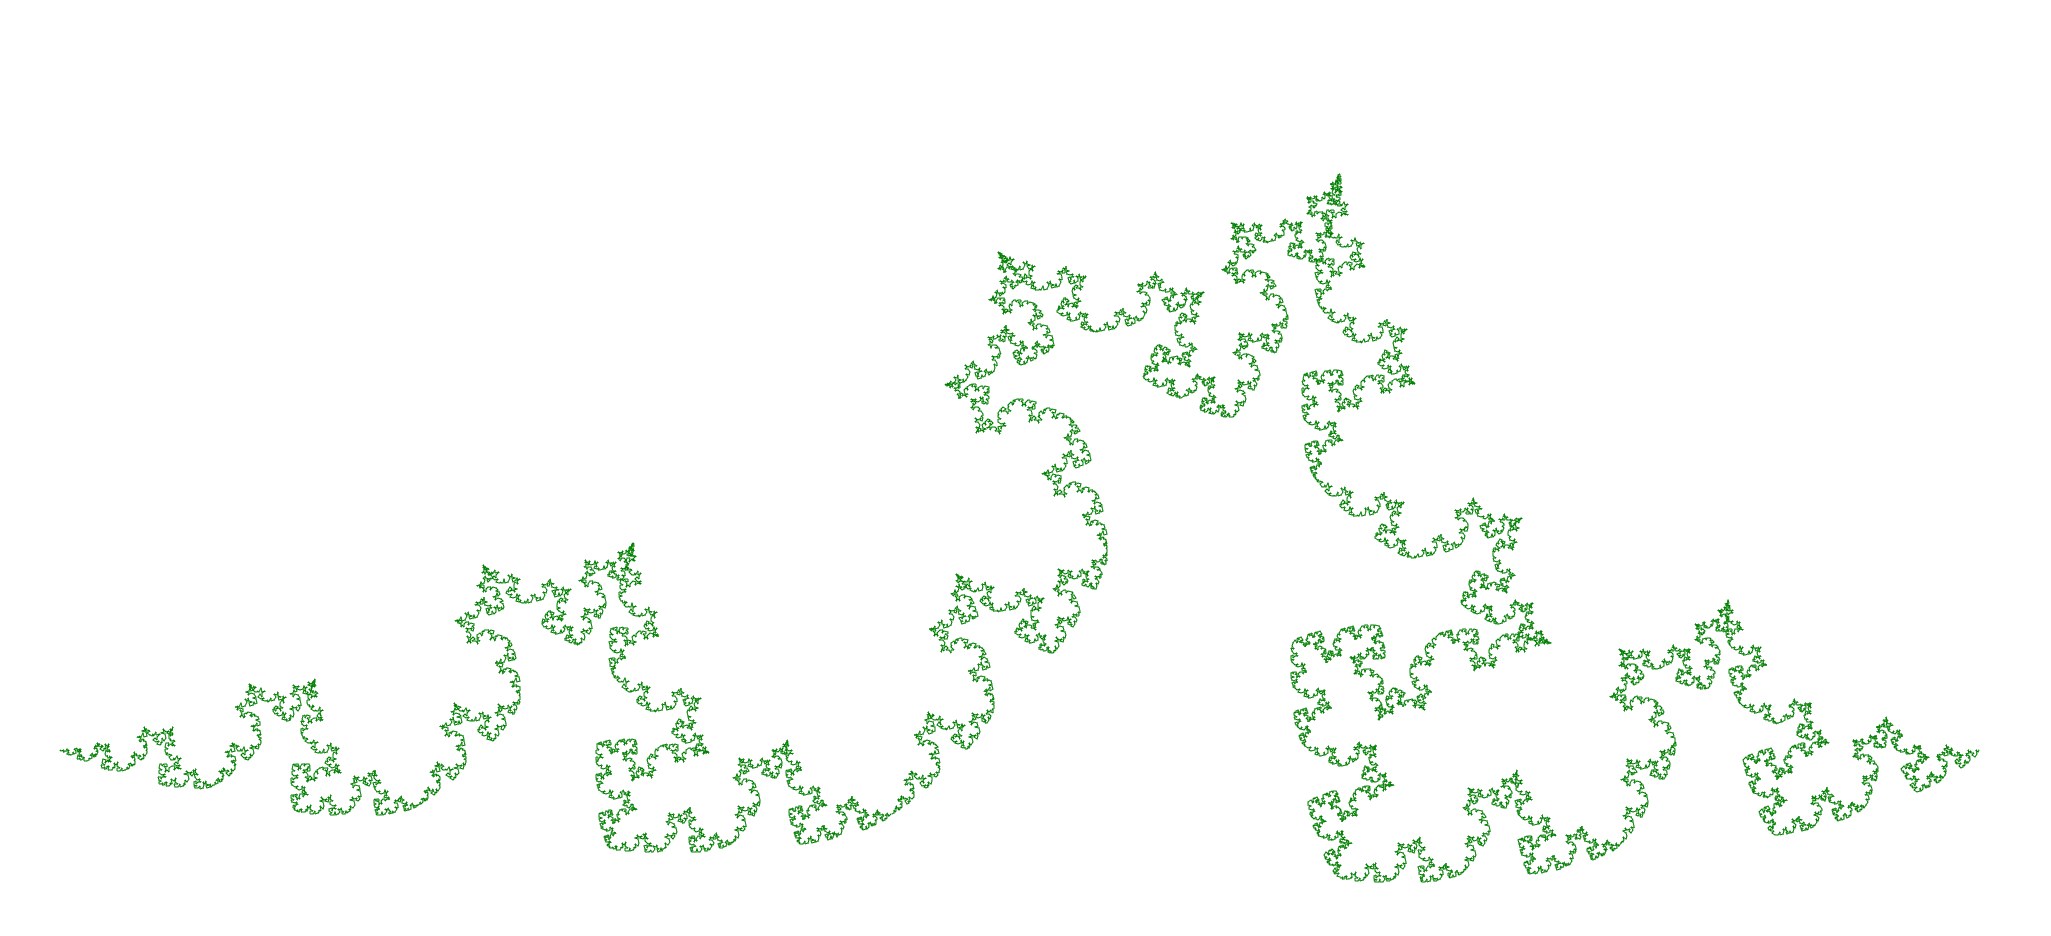
\includegraphics[width=0.49\textwidth]{img/Simple_Variations/koch_variation_03.png}
                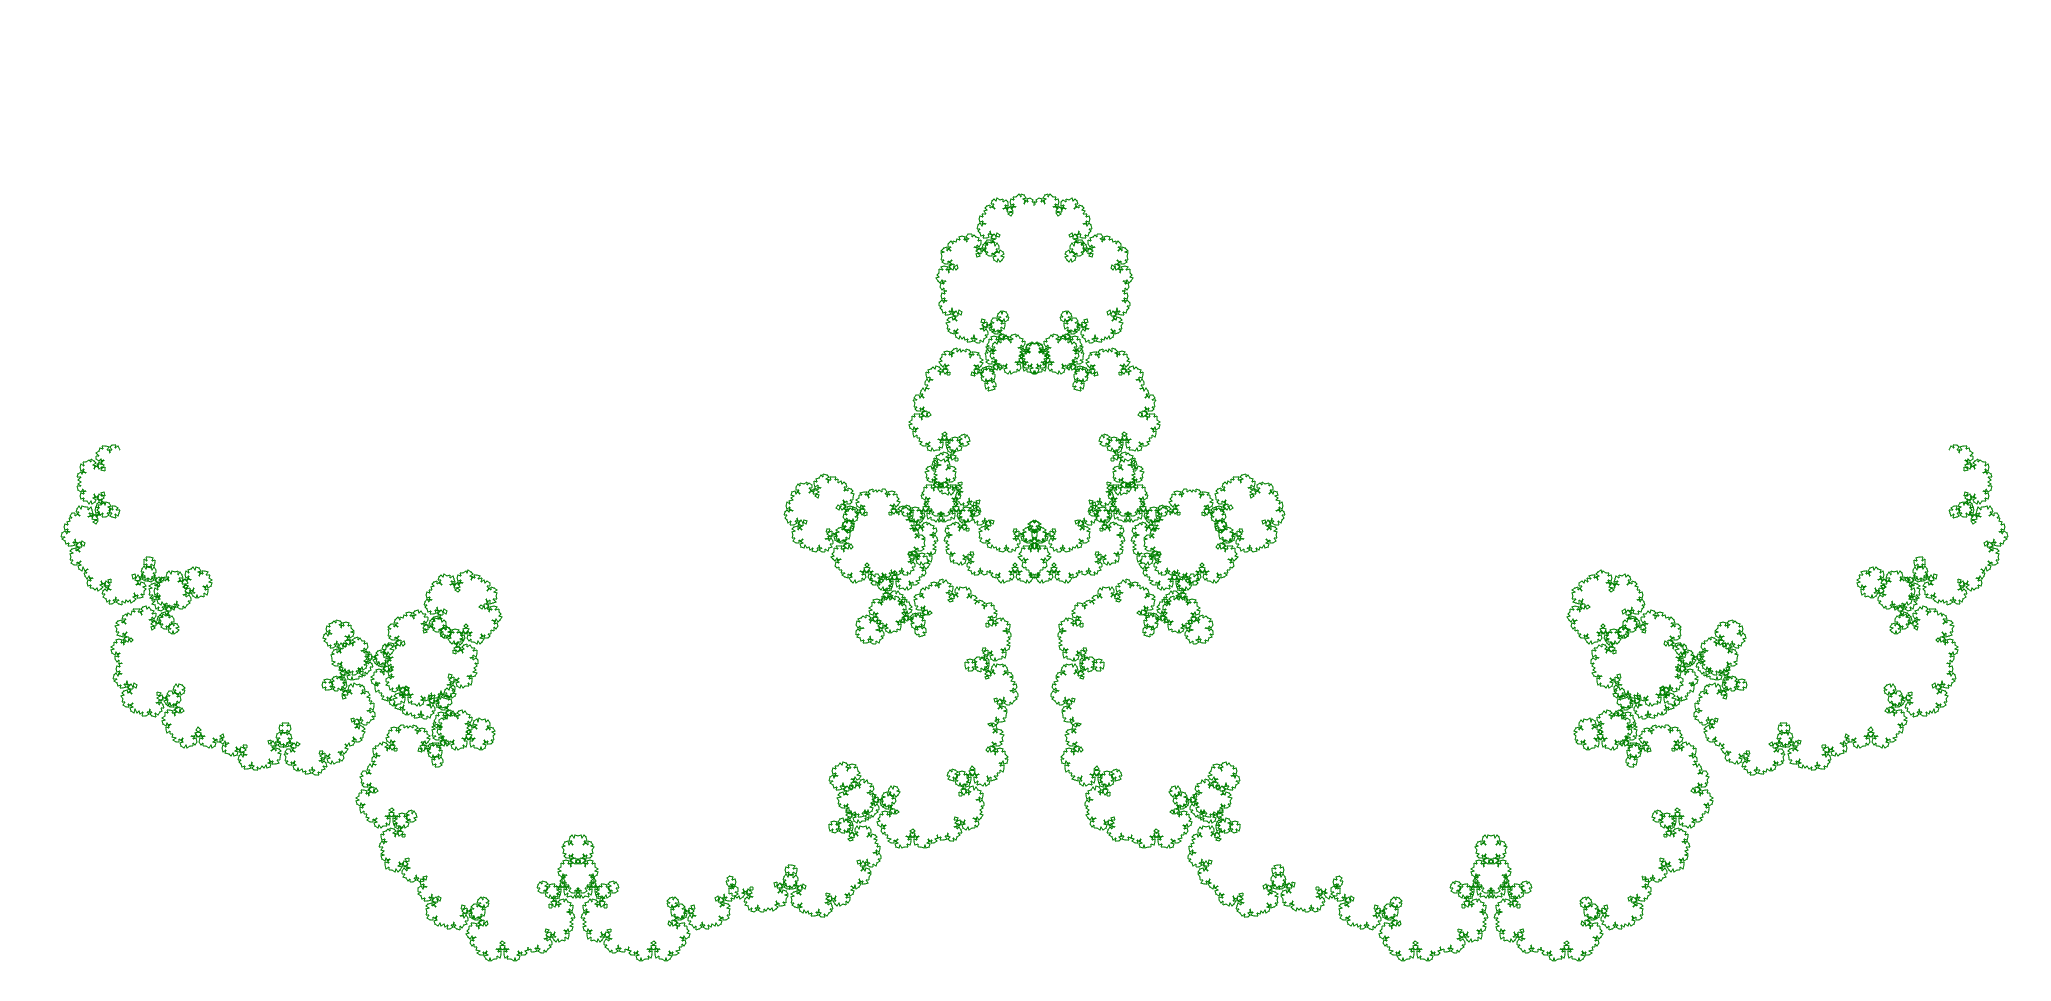
\includegraphics[width=0.49\textwidth]{img/Simple_Variations/koch_variation_04.png}
            \end{figure}

            \FloatBarrier
